\documentclass[]{scrartcl}
\usepackage{graphicx}

%opening
\title{2ary Structure Prediction}
\author{Guillermo Romero Moreno}

\begin{document}

\maketitle

\tableofcontents

\section{Intro}
\subsection{Motivation}
\subsubsection{Biological}
"After translation, proteins fold into a 3-dimensional structure, known as the tertiary structure (Fig. 3A)."\cite{Jurtz2017}

"Knowledge of a protein’s structure can help to understand its function. Therefore de novo prediction of protein structure from sequence is a problem of great biological interest (Dill and MacCallum, 2012)." \cite{Jurtz2017}

"An important step in the prediction of tertiary protein structure is the prediction of the secondary structure, the local conformations of the peptide back-bone." \cite{Jurtz2017}

"There are three main classes of secondary structure: alpha-helix, beta-strand and coil. These can be further divided into 8 classes (Kabsch and Sander, 1983) (3 sub-classes of helix, 2 sub-classes of strands and 3 sub-classes of coil)." \cite{Jurtz2017}

"The 3D structure of a protein is determined largely by its amino acid sequence1. However it is extremely challenging to predict protein structure from sequence alone2. Since protein structure is critical to analysis of its function and many applications like drug and/or enzyme design3–5, understanding the complex sequence-structure relationship is one of the greatest challenges in computational biology6–8. Accurate protein structure and function prediction relies, in part, on the accuracy of secondary structure prediction9–12. [...] Overall, protein secondary structure can be regarded as a bridge that links the primary sequence and tertiary structure and thus, is used by many structure and functional analysis tools15–18" \cite{Wang2016}

"Protein tertiary structure prediction from amino acid sequence is a very challenging problem in computational biology (Yaseen and Li, 2014; Dill and MacCallum, 2012). However, if a protein secondary structure can be predicted accurately, it can provide useful constraints for 3D protein structure prediction. Protein secondary structure can also help identify the protein function domains and may guide the rational design of site-specific mutation experiments (Drozdetskiy et al., 2015)." \cite{Fang2017}

"The three-dimensional structure is also known as native conformation and it is a function of its secondary structures. A number of diseases, including cancer, Alzheimer’s disease, cystic fibrosis, Huntington’s disease and diabetes are linked to the result of the aggregation of ill-formed proteins [1], [2]. Notwithstanding, despite a large number of proteins that have been discovered recently (around 84.8 million records in the UniProtKB/TrEMBL repository as in may/2017), only a few of them have their structure known (129,745 in the Protein Data Bank – PDB as in may/2017). Therefore, acquiring knowledge about the structure of proteins is an important issue, since such knowledge can lead to important medical and biochemical advancements and even to the development of new drugs with specific functionality [3], [2]. [...] A possible way to infer the full structure of an unknown protein is to determine secondary structures in it. However, the pattern formation rules of secondary structures of proteins are still not known precisely [3]." \cite{Hattori2017}

"Proteins perform a wide variety of molecular functions, and most of those functions are determined by the protein’s three-dimensional structures. The problem of predicting the three-dimensional structure of a protein, given only its linear sequence of residues, is crucially important due to the high cost of experimental protein structure determination and the low cost of DNA sequencing to obtain protein sequences. However, even with this importance it is a problem which has remained unsolved since its inception half a century ago (Gibson and Scheraga, 1967; Dill and MacCallum, 2012; Zhou et al., 2011). Due to the challenge of predicting three-dimensional protein structure, the problem is commonly divided into smaller, more achievable problems, in the hopes that their solutions will ultimately lead to the solution for three- dimensional structure prediction. One type of these sub-problems is the prediction of one-dimensional structural properties of proteins, which can be represented as a one-dimensional vector along the protein sequence. The most commonly predicted one-dimensional structure of proteins is secondary structure. Secondary structure prediction can be dated back to 1951 when Pauling and Corey proposed helical and sheet conformations of protein backbone based on hydrogen bonding patterns (Pauling et al.,1951). Secondary structure is a course-grained descriptor of the local structure of the polypeptide backbone." \cite{Heffernan2017}

"Protein-based interactions are responsible for controlling a variety of vital functions: they are critical in driving the immune system, regulating breathing and oxygenation, controlling aging and energy usage, and determining drug response, with a protein’s particular functional role determined by its structure (Breda et al., 2006; Guo, Ellrott, \& Xu, 2008). Over time, scientists have reached a consensus that a protein’s structure primarily depends on its amino acid sequence–local and long-range interactions between amino acid residues and their side-chains are both a cause and consequence of protein secondary and tertiary structure (Dill et al., 2008). This hypothesis has driven a decades-long effort, spanning multiple disciplines, to deduce how protein sequence determines a protein’s structural and functional properties (Dill et al., 2008; Anfinsen, 1977).

As the number of proteins with known sequence continues to outpace the number of experimentally determined secondary and tertiary structures (Huang, Liu, \& Weinberger, 2016), computational approaches to protein structure prediction become increasingly desirable. Computational tools that can handle large amounts of data while making sufficiently accurate predictions of secondary structures can potentially serve to mitigate the cost and time burden in the experimental determination of protein structures." \cite{Busia2017}

"There is a natural upper-bound on the maximum possible Q3 accuracy from inconsistencies in secondary structure assignment likely due to the coarseness and inherent arbitrariness of three-class labels (Kihara, 2005). This is likely also the case for the eight-class instantiation of the problem. A better approach might be to predict the sequence of back-bone angles for the amino acids, since these are experimentally observed values." \cite{Busia2017}

"Accurately and reliably predicting structures, especially 3D structures, from protein sequences is one of the most challenging tasks in computational biology, and has been of great interest in bioinformatics [Ashraf and Yaohang, 2014]. Structural understanding is not only critical for protein analysis, but also meaningful for practical applications including drug design [Noble et al., 2004]. Understanding protein secondary structure is a vital intermediate step for protein structure prediction as the secondary structure of a protein reflects the types of local structures (such as 310−helix and β−bridge) present in the protein. Thus, an accurate secondary structure prediction significantly reduces the degree of freedom in the tertiary structure, and can give rise to a more precise and high resolution protein structure prediction [Ashraf and Yaohang, 2014; Zhou and Troyanskaya, 2014; Wang et al., 2011]." \cite{Li2016}
\subsubsection{Computer software}
"slowly spreading into biology and bioinformatics. One potential cause of this is the lack of examples or code templates tailored to bioinformatics problems combined with the notion that the implementation and training of deep learning methods is complicated and computationally challenging" \cite{Jurtz2017}

"Other than the prediction accuracy, secondary structure prediction provides an ideal testbed for exploring and testing these state-of-the-art deep-learning methods, in a similar spirit of ImageNet (http://www.image-net.org) for deep-learning method development." \cite{Fang2017}

\subsection{Deep Learning}
"Since then improvements have been made in part enabled by the access to greater computational resources, especially graphics processing units (GPU), enabling training of deep neural networks containing many parameters in reasonable time. Given this, special- ized neural network architectures like convolutional neural net- works (CNN) and recurrent neural networks (RNN) with long short-term memory cells (LSTM) can now be trained efficiently and have been successfully applied to many problems" \cite{Jurtz2017}

"Recently, Deep-Learning (DL) gained attention with appli-
cations in several domains, such as speech recognition systems (the first major industrial application of DL), natural language understanding, sentiment analysis, language translation, image recognition, particle accelerator data analysis and Bioinfor- matics. Here, it is important to recall that it was possible with the advent of the Graphical Processing Units (GPUs). DL approaches are representation-learning methods with multiple levels of representation, from the raw input to a slightly more abstract level [22]. Basically, a DL architecture is composed by a stack of modules that are subject to learning with a large number of parameters. Moreover, it is known that large networks rarely present local minima. However, such networks are prone to overfitting. Also, training different architectures is very hard because finding an optimal set of hyper-parameters for each architecture is a difficult task and training each network is computationally expensive. [...] The training of deep networks was proved to be hard due to the variation of the backpropagated gradients at each time step, typically vanishing over several time steps [22]. Regarding this issue, [24] proposed a way to explore the use of rectifying non-linearities instead of using the well- known sigmoid and hyperbolic tangent functions, known as the Rectified Linear Units (ReLU), which is a better model of biological neurons and allows the network to obtain sparse representations. Nowadays, the ReLU is considered to be the most popular non-linear activation function. It is a half-wave rectifier f(x) = max(x, 0) (where x is the input to a neuron). The advantage of the ReLU, compared with other logistic functions, is that it learns much faster in multi-layer networks, allowing training of a deep supervised network [22]." \cite{Hattori2017}

\subsection{CNNs}
"In convolutional neural networks (CNNs) information also flows only from the input to the output, layer by layer. They are however not fully connected, but instead slide a filter (a set of weights) over the input that feeds into a different neuron in the next layer each time it is moved as illustrated in Figure 1B. The filter will thereby identify features in input irrespectively of where they appear. This concept is visualized in Figure 1C using the example of a convolutional filter detecting a motif in an amino acid sequence. Pooling such as mean pooling (averaging of nearby positions) enables the network to become invariant to small local de- formations in the input. Convolutional neural networks often consist of many convolutional filters and many convolutional and pooling layers to enable the network to integrate the information from the different filters and various levels of abstraction (LeCun et al.,2015). When applied to biological problems, convolutional neural networks are ideally suited to locate motifs, for example in a protein sequence, independent of their position within the sequence." \cite{Jurtz2017}

"Max-pooling provides a way of reducing the input or hidden layer size by selecting only the maximally activated neuron from a number of neighboring neurons. Alternatively mean pooling can be performed where the mean activation is calculated among neighboring neurons. Pooling is often used in convolutional neural networks (LeCun et al., 2015). To make a convolutional neural network independent of the input sequence length, global max-pooling can be applied where only the maximally activated neuron of the input or hidden layer is selected for each of the convolutional filters. In this way, the number of hidden neurons generated by the convolutional filters is equal to the number of filters and not influenced by the input sequence length." \cite{Jurtz2017}

"Each convolution layer consists of four consecutive operations: 1) The convolution operation with certain kernel size. 2) The batch normalization (Ioffe and Szegedy, 2015) operation is applied to help speed up
the training process and acts as a regularizer. 3) The activation operation, ‘ReLU,’ (Radford et al., 2015) was used as an activation function. 4) The dropout (Srivastava et al., 2014) operation to prevent the neural network from overfitting randomly drops neurons during the deep network training process such that the network can avoid too much co-adapting." \cite{Fang2017}

"The proposed Deep3I network (see Fig. 2) differs from the previous net- work (Li and Yu, 2016; Busia and Jaitly, 2017) in that the latter ones used residual blocks and multi-scale layer containing CNN layers with a convolution window size of 3, 7, and 9 to discover protein local and global context. Deep3I consists of stacked CNN layers, whose convolution window size is only 3. When stacked deep convolution blocks are put together, they can perform both local and global context extraction. Applying convolution on top of convolution, the sliding window will cover a wide range of protein sequences by using this hierarchical convolutional operation." \cite{Fang2017}
\begin{figure}[h]
	\centering
	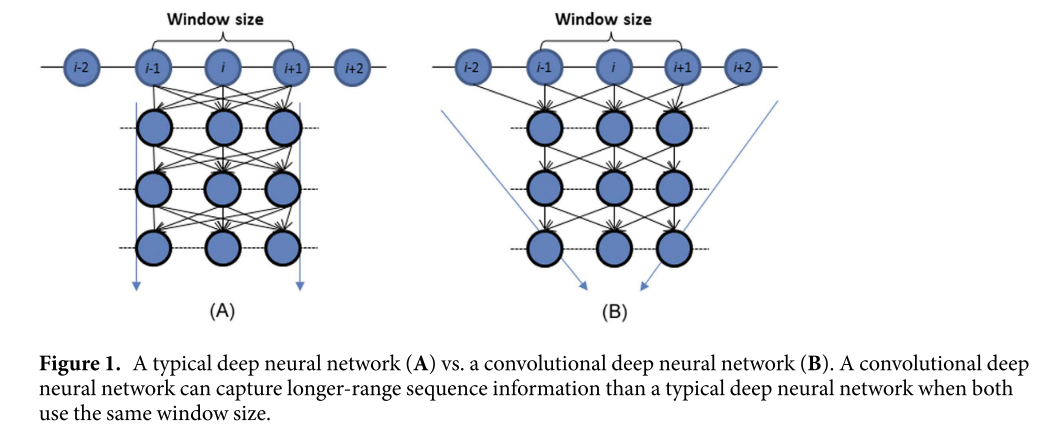
\includegraphics[width=1\linewidth]{cnnwang}
\end{figure}

"Although a fully-connected layer–where every input of interest is connected to every neuron in the layer by a distinct weight–is usually considered the simplest type of layer in a neural network, in some senses a convolutional layer can be thought of as a further simplification. Whereas fully-connected layers can be understood as an attempt to capture information from the inputs simultaneously by defining a large number of neurons with distinct weights, convolutional layers consist of filters–smaller groups of neurons– which look at segments of the input sequence at a time. Thus, a convolutional filter can be interpreted as sliding along the input sequence, reusing the same few weights on each local patch of the input. [...] The convolutional filters, CF and CF’, are defined by their width–the number of inputs examined at a time–and depth–the number of neurons in the filter. [...] one of the major benefits of convolutions compared to a the previous fixed-window, fully-connected approach: in situations where local properties of the data are critical, stacking small filters–each of which examines a small local input patch at a time–introduces the ability to learn and maintain information about sequence dependencies at different scales. [...] filters in lower layers focus on extracting information from small local contexts–in this case, of three residues–while filters in higher layers cover correlations which are more spatially spread-out in the input sequence." \cite{Busia2017}
\begin{figure}[h]
	\centering
	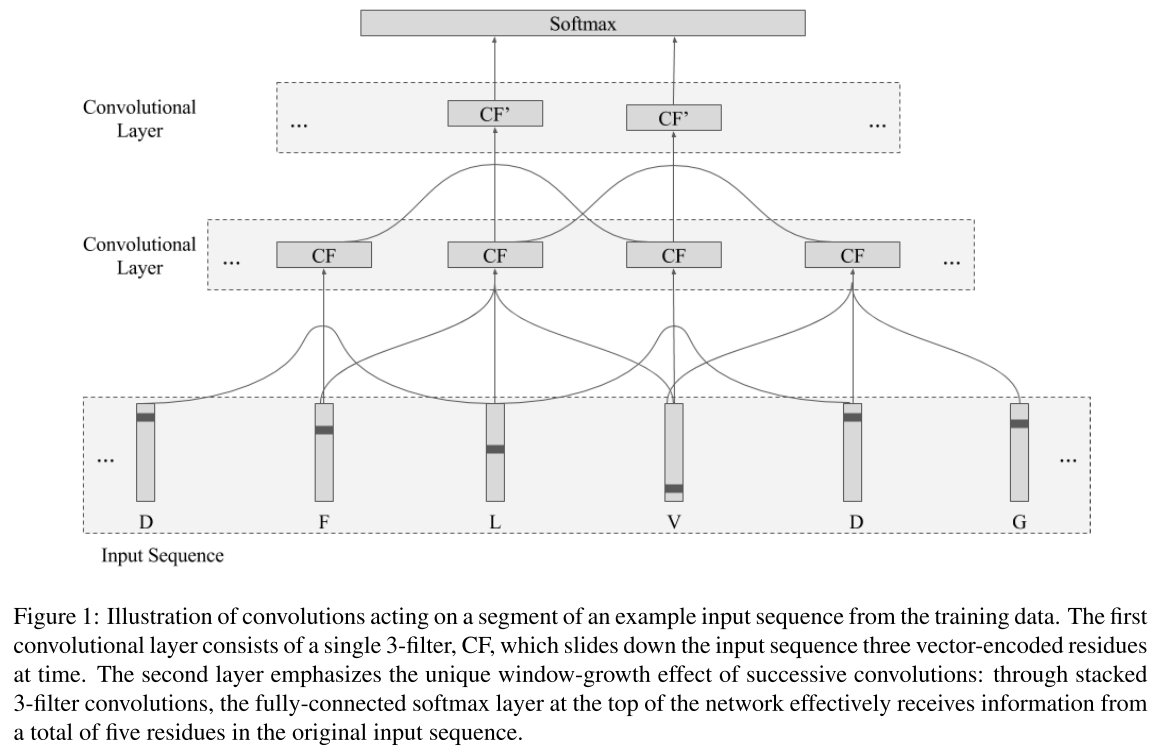
\includegraphics[width=1\linewidth]{stackedCNN}
\end{figure}

"Convolutional neural networks (CNN) [LeCun et al., 1998], a specific type of deep neural networks using translation-invariant convolutional kernels, can be applied to extracting local con- textual features and have proven to be effective for many natural language processing (NLP) tasks [Yih et al., 2011; Zhang et al., 2015]. Inspired by their success in text classification, in this paper, CNNs with various kernel sizes are used to extract multiscale local contexts from a protein sequence." \cite{Li2016}
\subsubsection{CNNs on biological sequencial data}
DeepCNF (section \ref{DeepCNF}) uses 2D convolutions of size window times feature vector size.
\begin{figure}[h]
	\centering
	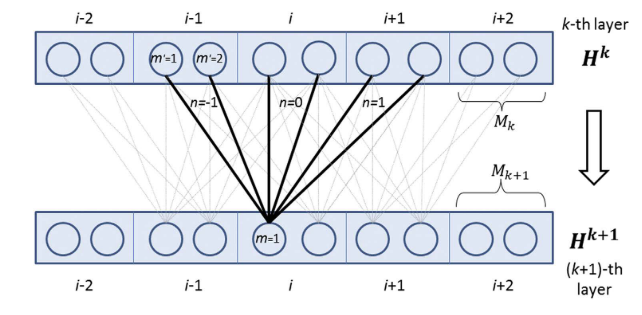
\includegraphics[width=0.7\linewidth]{DeepCNF}
	\caption{They implement convolution without knowing, so se hacen un pifostio intentando explicar la arquitectura.}
\end{figure}

"Amino Acids C, A, D, A, D are encoded as ‘one-hot’ vectors with a 1 at the position corresponding to the amino acid type (A, C or D), and zero otherwise. A filter (blue) is slid over the input sequence. The filter here has a length of three amino acids. At each position the filter has a preference for different amino acid types. The filter output is calculated by taking the sum of the element-wise product of the input and the filter position-specific weights. Each time the filter is moved, it feeds into a different hidden neuron in the hidden layer, here visualized in the f1 row. Multiple filters will give multiple inputs to the next layer {f1, f2, f3, ...}. A filter can be visualized as a sequence motif. This helps to understand which amino acids the filter prefers at each sequence position. When the filter is slid over the input sequence, it functions as motif detector and becomes activated when the input matches its preference. For example, this filter has negative output for sub-sequences ADC and positive for DCD." \cite{Jurtz2017}
\begin{figure}[h]
\centering
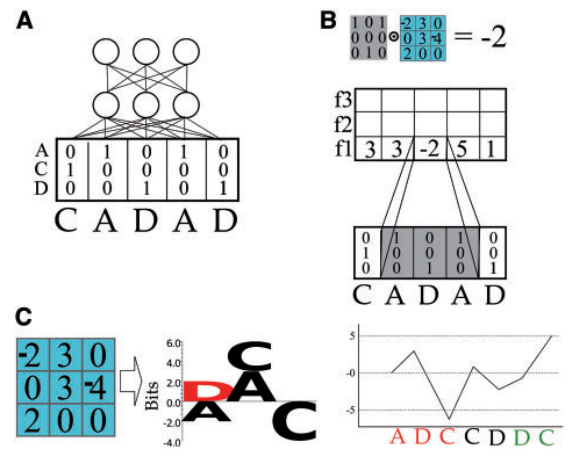
\includegraphics[width=0.7\linewidth]{cnnbio}
\label{fig:cnnbio}
\end{figure}

"Convolutional Neural Networks (CNNs) have been used to overcome the limitations of windowing by applying layers of shifting convolutional kernels across the input sequence (Wang et al., 2016). The addition of each subsequent convolutional layer includes a window of information from the layer prior. This has the effect of growing the size of the window being applied to the input data, each time a layer is added. However, even though the effective window size increases at each layer, the total window is still finite and limited. DeepCNF for example uses five CNN layers, each with a window size of 11 (five on either side), this is only able to capture information from residues plus or minus 25 sequence positions away." \cite{Heffernan2017}

\subsection{LSTMs}
"The purpose of Recurrent Neural Networks (RNN) is to
learn long-term dependencies. However, it is known that is difficult to learn to store information for very long [25]. One approach to correct for that is to augment the network with an explicit memory, called the Long Short-Term Memory (LSTM) network [26]. It was proposed for using special hidden units that lead to the natural behaviour of remembering inputs for a long time, known as memory cells. In other words, the gradient can flow for long time, thereby avoiding the vanishing gradient problem. Figure 2 1 shows a memory cell, which is an accumulator that has a connection to itself at the next time step. Basically, the LSTM process is composed by three gates (i.e. the forgot gate ft, update gate it and output gate ot ). The variables xt and ht represent the input and output of the network at time t. The layers with sigmoid and hyperbolic tangent activation functions are represented by σ and tanh." \cite{Hattori2017}

"Bidirectional Recurrent Neural Networks (BRNNs) (Schuster and Paliwal, 1997) can exploit both preceding and following dependencies across the whole sequence and have been used in a number of bioinformatic studies (Baldi et al., 1999; Pollastri et al., 2002a; Mirabello and Pollastri, 2013; Magnan and Baldi, 2014). Long Short-Term Memory (LSTM) cells were introduced to be able to learn both local and non-local intra-sequence relationships more efficiently (Hochreiter and Schmidhuber, 1997). In recent years, LSTM-based networks have enjoyed significant success in a wide variety of tasks that involve learning from sequences, from speech recognition (Amodei et al., 2015), to natural language processing (Sundermeyer et al., 2012), and handwriting recognition (Graves and Schmidhuber, 2009). Its recent application to protein intrinsic disorder prediction demonstrates its ability to capture non-local interactions in protein sequences (Hanson et al., 2017)" \cite{Heffernan2017}

"Similar to CNNs, recurrent neural networks (RNNs) are another specific type of neural networks with loop connections. They are designed to capture dependencies across a distance larger than the extent of local con- texts. In previous work [Sepideh et al., 2010], RNN models could not perform well on protein secondary structure prediction partially due to the difficulty to train such models. Fortunately, RNNs with gate and memory structures, including long short term memory (LSTM) [Hochreiter and Schmidhuber, 1997], gate recurrent units (GRUs) [Cho et al., 2014a], and JZ3 structure [Jozefowicz et al., 2015], can artificially learn to remember and forget information by using specific gates to control the information flow. In this paper, we exploit bidirectional gate recurrent units (BGRUs) to capture long-range dependencies among amino acids from the same protein sequence." \cite{Li2016}

\subsection{Framework}
"The successes of neural networks have led to the development of various programming frameworks to build and train neural net- works. Examples are PyTorch (http://pytorch.org/), Caffe (http:// caffe.berkeleyvision.org) and TensorFlow (https://www.tensorflow. org). Our framework of choice here is Lasagne (Dieleman et al., 2015), a well-established easy to use and extremely flexible light- weight Python library built on top of the Theano numerical compu- tation library (Bastien et al., 2016). While most other frameworks require the user to learn a dedicated programming language, Lasagne is Python-based and therefore relatively easy to use for bio- informaticians already programming in Python. Further Lasagne’s active community ensures that the latest neural network training al- gorithms and architectures are available to the user." \cite{Jurtz2017}

"TensorFlow 1.0 (Abadi et al., 2016) and Keras 2.0 (Chollet, 2015; https://github.com/fchollet/keras) were used for the training of the deep learning." \cite{Fang2017}

"The software was developed using the Python programming language and the Lasagne framework 3." \cite{Hattori2017}

"We use Google’s open-sourced TensorFlow library (Abadi et al., 2016) to implement and train our networks." \cite{Heffernan2017}

"Our models are implemented using TensorFlow, an open-source machine learning software library available at TensorFlow.org." \cite{Busia2017}
\subsubsection{Lasagne}
"Lasagne is a lightweight library to build and train neural networks (Dieleman et al., 2015). It is written in the Python programming language (Python Software Foundation, Python Language Reference, version 2.7) and built on top of another library called Theano (Bastien et al., 2012), which allows the user to define, optimize and evaluate mathematical expressions and most importantly for neural network training it implements efficient symbolic differentiation. Another key advantage of Theano, which is also inherited by Lasagne, is that it makes using a GPU easy and transparent.

Lasagne is being constantly updated, providing its users with an easy way to implement and test the newest neural network architectures and training procedures. At the time of writing, the Lasagne library contains feed forward, convolutional and recurrent layers, various activation functions and many options for weight initialization and gradient descent optimizers including Nesterov momentum, RMSprop and ADAM (Kingma and Ba, 2014). 

The Lasagne documentation includes a tutorial and other code examples in a recipe directory." \cite{Jurtz2017}

\subsection{Open-source}
"We developed the first open-source deep-learning based secondary structure prediction tool MUFold-SS. It was implemented and provided to the research community. The open source advantage adds significant value to this work, as it allows other researchers to easily apply this deep-learning framework for many other research problems." \cite{Fang2017}


\section{Problem definition}
\subsection{Local and non-local interactions}
"This suggests that a large portion of the information relevant to predicting an amino acid’s secondary structure arises from the local interactions amongst relatively few of the directly neighboring residues, with the recurrent layers in Li \& Yu (2016) model learning relatively little additional information from the remainder of the input sequence." \cite{Busia2017}

"It is well known that local contexts are critical for protein secondary structure prediction. Specifically, the secondary structure category information of the neighbours of an amino acid are the most effective features for classifying the secondary structure this amino acid belongs to. [...] On the other hand, long-range interdependency among different types of amino acids also holds vital evidences for the category of a secondary structure, e.g., a β−strand is steadied by hydrogen bonds formed with other β−strands at a distance [Zhou and Troyanskaya, 2014]." \cite{Li2016}

\subsection{Datasets}
\subsubsection{CullPDB53}
CullPDB (Wang and Dunbrack, 2003)
6125 proteins
"The CullPDB dataset was constructed before CASP10 (i.e., May 2012) and any two proteins in this set share less than 25\% sequence identity with each other." \cite{Wang2016}

"The CullPDB data set from Zhou and Troyanskaya, (2014) was constructed before January 2014, and any two proteins in this set shared less than 25\% sequence identity with each other. This CullPDB contained 6128 proteins. The filtered data set of this CullPDB had a sequence identity of less than 25\% with the CB513 test data, and it contained 5534 protein sequence after filtering." \cite{Fang2017}

"We trained all neural networks on the cullpdb+profile\_6133\_filtered dataset (http://www.princeton.edu/~jzthree/datasets/ICML2014/). [...] The dataset consists of amino acid sequences of proteins with a length up to 700 amino acids and corresponding sequence profiles. [...] The original training set consists of 6133 sequences, but was been filtered to remove sequences that shared more than 30\% identity with sequences in the CB513 dataset." \cite{Jurtz2017}

"We use two publicly available benchmark datasets, pre-processed by Zhou \&Troyanskaya (2014)∗: CullPDB and CB513. Each of these consists of protein sequences and structure label assignments downloaded from the Protein Data Bank archive (PDB) (Berman, Henrick, \& Nakamura, 2003). [...] The full CullPDB dataset contains 6,128 proteins with less than 30\% sequence identity. Here, we use a subset of these data, which has been filtered to reduce sequence identity with the CB513 test data to at most 25\%. The resulting subset consists of 5,534 protein sequences–or equivalently 1,183,318 individual amino acid residues– for prediction. Consistent with Sønderby \& Winther’s (2014) arrangement, we randomly divide these 5,534 proteins into a training set of 5,278 proteins and a validation set of 256 proteins." \cite{Busia2017}
\subsubsection{CB513 \& CB6133}
"Experimental results on the CB6133 dataset, the public CB513 benchmark" \cite{Li2016}

"CB513 benchmark used in Zhou and Troyanskaya (2014), Wang et al. (2016), Li and Yu (2016), and Busia and Jaitly (2017). This benchmark was widely used and was chosen from secondary structure tools for performance comparison." \cite{Fang2017}

"two datasets with 8 classes of secondary structure were used: the so-called CB6133 [19] and CB513 datasets [20]. The CB6133 has 6133 protein sequences (in- stances) and the CB513 has 513 instances which, in turn, were included in the CB6133 dataset. The CB6133 (excluded the CB513 intances) was used in the training (5278 instances) and validation (256 instances) tasks, as in [16]. On the other hand, the CB513 was used for testing the network with 513 instances" \cite{Hattori2017}

"The CB513 dataset was first published by (Avdagic et al., 2009), the version with additional profile encoding we use is based on (Zhou and  Trojanskaya, 2014) (http://www.princeton.edu/~jzthree/datasets/ICML2014/)." \cite{Jurtz2017}

"We use two publicly available benchmark datasets, pre-processed by Zhou \&Troyanskaya (2014)∗: CullPDB and CB513. Each of these consists of protein sequences and structure label assignments downloaded from the Protein Data Bank archive (PDB) (Berman, Henrick, \& Nakamura, 2003). [...] The 513 protein sequences in the CB513 dataset are used exclusively to measure test Q8 accuracy–that is, the percentage of the 84,765 amino acid residues for which the predicted secondary structure labels are correct." \cite{Busia2017}

\begin{figure}[h]
	\centering
	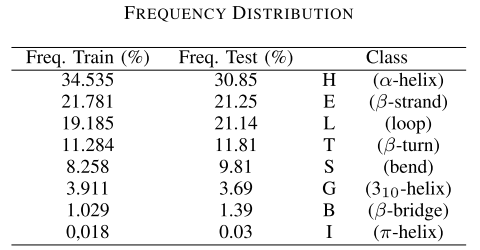
\includegraphics[width=0.5\linewidth]{targetfreq}
	\caption{Target frequencies on the CB6133 (left) and the CB513 (right).}
	\label{fig:targetfreq}
\end{figure}
\subsubsection{CASP 10, 11 \& 12}
123 domain sequences
105 domain sequences
"the recent CASP10 and CASP11 datasets" \cite{Li2016}

"Critical assessment of protein structure prediction (CASP) is a community-wide protein structure prediction bi-annual competition. CASP targets were widely used for benchmark protein prediction tools. [...] CASP 10, 11, and 12 were downloaded on May 2012, 2014 and 2016." \cite{Fang2017}

"Each protein from the CASP data set was stored in the PDB format. To prepare the data set, the PDB files were downloaded from the official CASP website under the target directory: http://prediction-center.org/download\_area/CASP10/targets/.
Note that some of the PDB files provided do not cover the corresponding FASTA file. For example, the T0644.fasta contains 166 amino acids; however, the T0644.pdb con- tains only 141 amino acids. To be more consistent, the extracted sequence from PDB provided by CASP was used. The DSSP program (Touw et al., 2015; Kabsch and Sander, 1983) was used to get the secondary structure label from the PDB files. Some of the PDB files (T0675, T0677 and T0754) could not generate the DSSP results, and they were discarded. Some protein sequences (T0709, T0711, T0816 and T0820) are too short and PSI-BLAST did not have a hit; hence, they could not be considered in the evaluation, either. Overall, the effective proteins used are CASP10 (98 out of 103), CASP 11 (83 out of 85) and CASP 12 (40 out of 40)." \cite{Fang2017}
\subsubsection{CAMEO}
http://www.cameo3d.org/sp/6-months/
"403 CAMEO test targets, test proteins in the past 6 months (from 2014-12-05 to 2015- 05-29)." \cite{Wang2016}
\subsubsection{JPRED}
"publically available JPRED training and test data47 (http://www.compbio. dundee.ac.uk/jpred4/about.shtml), which has 1338 training and 149 test proteins, respectively, each of which belongs to a different superfamily." \cite{Wang2016}

"we retrained our DeepCNF models using the 1338 JPRED training proteins and tested the resultant models on the 149 JPRED test proteins47. All the test and training proteins belong to different superfamilies. That is, it is unlikely that one test protein shares similar sequence profile with one training protein. The sequence profiles of these JPRED training and test proteins are generated from an NR database dated in 2012- 10-26." \cite{Wang2016}

"JPRED (Drozdetskiy et al., 2015) data set. This benchmark contains non-redundant proteins for training and testing, and each of the protein belongs to a different superfamily." \cite{Fang2017}

\subsubsection{Wang}
"Meanwhile, datasets (2-5) are only used for test. [...] Following the same procedure in36, we divided CullPDB into two subsets for training and test, respectively, such that the training proteins share no more than 25\% sequence identity with our test sets (2-4). Our training set consists of ~5600 CullPDB proteins and the remaining ~500 PDB proteins are used as the test data. In total there are 403 CAMEO test targets in the past 6 months and 179 proteins are kept for test after removing those sharing more than 25\% sequence identity with the training set.
The native SS labels of all the training and test proteins are generated by DSSP14.
An alternative way to select non-redundant proteins for training and test is to pick one representative from each protein superfamily defined by CATH56 or SCOP57. By using test proteins in different superfamilies than the training proteins, we can reduce the bias incurred by the sequence profile similarity between the training and test proteins. To fulfill this, we use the publically available JPRED training and test data47 (http://www.compbio.dundee.ac.uk/jpred4/about.shtml), which has 1338 training and 149 test proteins, respectively, each of which belongs to a different superfamily." \cite{Wang2016}
\subsubsection{Fang}
"In this work, four public data sets were used: 1) CullPDB (Wang and Dunbrack, 2003) used in Zhou and Troyanskaya (2014) and Busia and Jaitly (2017). The CullPDB data set from Zhou and Troyanskaya, (2014) was constructed before January 2014, and any two proteins in this set shared less than 25\% sequence identity with each other. This CullPDB contained 6128 proteins. The filtered data set of this CullPDB had a sequence identity of less than 25\% with the CB513 test data, and it contained 5534 protein sequence after filtering. Finally, 5278 protein sequences were randomly chosen from the filtered CullPDB to form a training set, and the remaining 256 sequences formed the validation set.
2) CB513 benchmark [...]
3) JPRED [...]
4) CASPs 10, 11 and 12 [...]

The data set (1) was used to train the deep network while data sets (2–4) were only used for testing and comparison with other state-of-the-art tools. \cite{Fang2017}
\subsubsection{SPIDER3}
"we employed exactly same datasets as used in our previous studies (Lyons et al., 2014; Heffernan et al., 2015, 2016). The full dataset contains 5789 proteins with a sequence similarity cut off of 25\% and X-ray resolution better than 2.0 A˚ . From the full set of data, 4590 proteins were randomly selected to be the training set (TR4590), and the remaining 1199 are used as the independent test set (TS1199). The TR4590 set is further split into a training and validation set (TR4131 and VAL459, respectively) so that the validation set can be used for early stopping during training. [...] In addition, we obtained all the high-resolution (<3A˚ ) proteins deposited in 2016 (prior to September 16, 2016) that are below 30\% sequence similarity among each other and to all proteins deposited prior to 2016. This constitutes a separate independent test set of 115 proteins." \cite{Heffernan2017}

\subsection{Features}
"The input features we used are the same as (Busia and Jaitly, 2017). The amino acid at position i is represented as one-hot vector. There are 20 different types of amino acids. Some special amino acid cases were handled as follows: Amino Acid ‘X’ was treated as amino acid ‘A’. ‘B’ was treated as amino acid ‘N’. ‘Z’ was treated as amino acid ‘Q’. Since the input size was fixed at 700, if the input protein sequences were less than 700 amino acids; the remaining amino acid positions were padded with the ‘NoSeq’ label, which means no amino acid was there. Current implementation can handle any protein sequence length less or equal to 700 amino acids. The protein sequences will be split into smaller segments if they have more than 700 amino acids. [...] The profile information is also represented as 700-by-21 array. Hence, the input dimension is 700-by-42 in total." \cite{Fang2017}

"each amino acid (ai) of the sequence (with n amino acids) has 42 features: 22 profile features are used for representing scores obtained from a Position-Specific Scoring Matrix (PSSM) [21], which are normalized using the logistic Sigmoid function. The last 20 features are used for representing the amino acid, using the one-hot encoding. In this encoding, only one bit is set and represents the name category of the amino acid." \cite{Hattori2017}

"amino acid was encoded using one-hot encoding and additionally a sequence profile." \cite{Jurtz2017}
\begin{figure}[h]
	\centering
	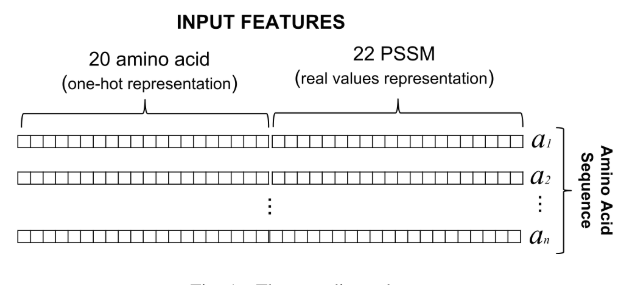
\includegraphics[width=0.7\linewidth]{features}
	\label{fig:features}
\end{figure}
"the first set of predictors take seven representative physio-chemical properties (PP) of amino acids (Fauche`re et al., 1988), 20-dimensional Position Specific Substitution Matrices (PSSM) from PSI-BLAST (Altschul et al., 1997), and 30-dimensional hidden Markov Model sequence profiles from HHBlits (Remmert et al., 2012) per residue as input [...] These features were selected previously in the development of SPIDER for secondary structure and contact prediction (Lyons et al., 2014; Heffernan et al., 2016, 2015). [...] The outputs from iteration 1 are then added to the PSSM, PP and HMM profile features, as inputs to a second set of predictors (iteration 2). This process is repeated two more times (iterations 3 and 4), for a total of four sets of networks as the result converges. [...] The TR4950 set is split into the same 10 folds for training every iteration of the network." \cite{Heffernan2017}

"Each protein is represented as a sequence of amino
acids, padded if necessary by no-sequence tokens to a sequence length of 700 residues. In turn, each amino acid is encoded as a 42-dimensional vector: the first twenty-one dimensions represent the one-hot encoding of the residue’s identity (or the no-sequence token), while the remaining dimensions contain Position-Specific Scoring Matrices (PSSM) generated with PSI-BLAST (see Zhou\&Troyanskaya (2014) for more details) which we normalize via mean-centering and scaling by the standard deviation." \cite{Busia2017}

"Overtime, scientists have reached a consensus that a protein’s structure primarily depends on its amino acid sequence and concluded that the local and long-range interaction are a cause of protein second and tertiary structure. Based on this hypothesis, we can deduce that proteins with similar amino acid sequence tend to have similar secondary structure sequence. Therefore, the common sequence information contained by PSSM can contribute to the secondary structure prediction. For a protein with length L, PSSM is usually represented as a matrix with L ×21 dimensions where 21 denotes the 20 standard types of residues and one extra residue type which represents all non-standard residue types. Before PSSMs are used in- puts for CNNH\_PSS, they need to be transformed to 0–1 range by the sigmoid function. By concatenating sequence features and evolutional information, each residue in protein sequences can be encoded by a feature vector with dimension of 42." \cite{Zhou2018}
\subsubsection{Beyond one-hot}
"the input feature sequence X is decomposed into two parts, one is a sequence of 21-dimensional feature vectors encoding the types of the amino acids in the protein and the other is a sequence of 21-dimensional profile features obtained from the PSI-BLAST [Altschul et al., 1997] log file and rescaled by a logistic function [Jones, 1999]. Note that each feature vector in the first sequence is a sparse one-hot vector, i.e., only one of its 21 elements is none-zero, while a profile feature vector has a dense representation. In order to avoid the in- consistency of feature representations, we adopt an embed- ding operation from natural language processing to transform sparse sequence features to a denser representation [Mesnil et al., 2015]. This embedding operation is implemented as a feedforward neural network layer with an embedding matrix, Wemb ∈ R21×Demb, that maps a sparse 21-dimensional vector into a denser Demb-dimensional vector. In this paper, we empirically set Demb = 50, and initialize the embedding matrix with random numbers. The embedded sequence feature vector is concatenated with the profile feature vector before being fed into multiscale CNN layers." \cite{Li2016}

"As the dimension of amino acid representation is already low, we only calculate a real value for every dimension by embedding technique and don’t decrease the dimension. The residue embedding in this paper is implemented by a feedforward neural net- work layer before multi-scale CNN in CNNH\_PSS [42]." \cite{Zhou2018}

"The protein sequence input is one-hot vector, which is a sparse matrix. In the future work, ProtVec (Asgari and Mofrad, 2015) will be explored to represent the sequence so that it will become a much denser and picture-like matrix, which may improve the Q3 and Q8 accuracy." \cite{Fang2017}

\subsection{PSI-BLAST profiles}
"PSI-BLAST generates a PSSM of size T × 20 for a T lengthed sequence, where a higher score represents a higher likelihood of the ith amino acid replacing the current one in other species. Generally, two amino acids that are interchangeable in the PSSM indicates that they are also interchangeable in the protein without sig- nificantly modifying the functionality of the protein." \cite{Lin2016}

"The BLOSUM matrix captures information about which pairs of amino acids are eas- ily interchangeable during evolution, but it does not capture information about the evolutionary constraints on a protein family (i.e. which amino acid positions are highly conserved and which are variable). This information can effectively be captured in a sequence profile. A sequence profile has the dimensions protein length times the number of amino acids and is conventionally generated by run- ning PSI-BLAST (Altschul et al., 1997) against a reference database. Encoding protein sequences as such profiles has demonstrated very helpful for prediction of for instance secondary structure (Jones, 1999)." \cite{Jurtz2017}

"DeepCNF has no significant advantage over the others when a protein under prediction has very sparse sequence profile (i.e., Neff ≤ 2). That is, it is still challenging to predict SS structure from primary sequence instead of sequence profile." \cite{Wang2016}

"We used the input features described in36. In particular, for each protein sequence, we ran PSI-BLAST41 with E-value threshold 0.001 and 3 iterations to search UniRef9079 to generate the position specific scoring matrix (PSSM). We then transform PSSM by the sigmoid function 1/(1 + exp(− x)) where x is a PSSM entry. We also use a binary vector of 21 elements to indicate the amino acid type at position i. We use 21 since there might be some unknown amino acids in a protein sequence. In total there are 42 input features for each residue, 21 from PSSM and the other 21 from the primary sequence. Note that besides using PSSM generated by 3 iterations, we could also add the PSSM generated by 5 iterations into the input features." \cite{Wang2016}

"A protein sequence is represented as a 700-by-21 array in the system. Next, protein profiles were generated using PSI- BLAST (Altschul et al., 1997), as performed in some previous work (Wang et al., 2016; McGuffin et al., 2000). The PSI-BLAST tool param- eters were set as follows: evalue: 0.001, num\_iterations: 3, db, and UniRef50 to generate a position-specific scoring matrix (PSSM). PSSM is then transformed by the sigmoid function so that the value is in range (0,1)." \cite{Fang2017}

"profile search time is relatively shorter than current available tools because we used a filtered version of the UniRef50 database. [...]
The PSI-BLAST can generate the protein sequence profile in a short time if the search database is small, while a larger search database takes a longer time to get the profile and the prediction accuracy may not always increase. [...] Four different databases were downloaded from UniProt
(http://www.uniprot.org/downloads). They are Swiss\_Prot (0.08GB), UniRef50 (4.3GB), UniRef90 (12GB) and UniRef100 (25GB). Take the UniRef50 database as an example: This database was used to perform a PSI-BLAST search with the parameter setup of evalue 0.001 and num\_iterations 3 on all protein sequences in the JPRED data set. Then, the train-ing set was used to train the Deep3I network, and the test set was used to report Q3, as shown in Table 1. The UniRef50 yielded the best results as a larger database was not needed to yield a better performance." \cite{Fang2017}

"The PSI-BLAST search database is UniRef50 and evalue is set to 0.001. Four experiments were performed with different num\_iteration of PSI-BLAST ranging from 2 to 5. Table 2 shows that too few or too many PSI-BLAST iterations do not yield good profile. The number of iterations of PSI-BLAST should be set to 3." \cite{Fang2017}

"Based on the information presented thus far, one could assume that the smaller the database, the better the Q3. One might ask: What will happen if an even smaller database is used for a PSI-BLAST search? To find out, we filtered a UniRef50 data set and kept those protein sequences whose length fell between 70 and 3000 thereby forming the shrunk database, UniRef50\_shrunk. Some other smaller databases were built, as shown in Table 3. Table 4 shows that the UniRef50\_smaller was sufficient for PSI- BLAST to use as a database and saves computing time. But when the da- tabase became even smaller, the prediction accuracy started to drop or fail. Another option would be to apply CD-Hit to shrink the database with a lower sequence similarity threshold" \cite{Fang2017}

\subsection{Targets}
"Pauling et al. (1951) proposed the earliest concept of protein secondary structure determining that the poly-peptide backbone contains regular hydrogen-bonded geometry, forming α-helices and β-sheets." \cite{Fang2017}

"Protein secondary structure (SS) refers to the local conformation of the polypeptide backbone of proteins. There are two regular SS states: alpha-helix (H) and beta-strand (E), as suggested by Pauling13 more than 60 years ago, and one irregular SS type: coil region (C). [...] Overall, protein secondary structure can be regarded as a bridge that links the primary sequence and tertiary structure and thus, is used by many structure and functional analysis tools15–18" \cite{Wang2016}
\subsubsection{Q3}
"(ssp) A collapsed version of the 8 class prediction task, since many protein secondary structure prediction algorithms use a 3 class approach instead of the 8-class approach given in dssp. {H, G} → H =Helix, {B, E} → B =Beta sheet, and {I, S, T, L} → C =Coil" \cite{Lin2016}

"The secondary structures (SS) of a protein represent the local conformations of a three-dimensional structure. There are three main secondary structures: α-helices [8], β-sheets [9] and turns [10]. For instance, proteins 1DG2 and 1KFP represent an α−helix and an β −sheet, respectively." \cite{Hattori2017}

"approaching the theoretical limit in the range of 88–90\% (Rost, 2001)." \cite{Heffernan2017}

"we predict three states by converting the DSSP assigned states G, H, and I to H; B and E to E; and S, T, and C to C." \cite{Heffernan2017}
\subsubsection{Q8}
"The class labels are H = alpha helix, B = residue in isolated beta bridge, E = extended strand, G = 3-helix, I = 5-helix, T = hydrogen bonded turn, S = bend, L = loop." \cite{Lin2016}

"The Q8 accuracy is another evaluation metric to evaluate the accuracy of eight-class classification: 310-helix (G), ?-helix (H), ?-helix (I), ?-strand (E), ?-bridge (B), ?-turn (T), bend (S) and loop or irregular (L) (Yaseen and Li, 2014; Zhou and Troyanskaya, 2014)." \cite{Fang2017}

"Sander14 developed a DSSP algorithm to classify SS into 8 fine-grained states. In particular, DSSP assigns 3 types for helix (G for 310 helix, H for alpha-helix, and I for pi-helix), 2 types for strand (E for beta-strand and B for beta-bridge), and 3 types for coil (T for beta-turn, S for high curvature loop, and L for irregular)." \cite{Wang2016}

"The DSSP program (Touw et al., 2015; Kabsch and Sander, 1983) was used to get the secondary structure label from the PDB files." \cite{Fang2017}

"Instead of using three classes, [11] group the secondary structures into 8 classes, including others, such as 310-helix, π-heliX and β- bridge." \cite{Hattori2017}

"The secondary structure of the proteins, which should be predicted, is given as eight different DSSP classes (Q8) (Kabsch and Sander, 1983). The dataset was originally downloaded from PDB and annotated with the DSSP program (Kabsch and Sander, 1983)." \cite{Jurtz2017}

"During training both of these networks mask out the loss contributed by any undefined labels, such as residues with no secondary structure assignment according to the program Dictionary of Secondary Structure of Proteins (DSSP) (Kabsch and Sander 1983)." \cite{Heffernan2017}

"DSSP (Kabsch and Sander, 1983) specifies eight secondary structure states. Three helix shapes: 310-helix G, alpha-helix H, and pi-helix I; two strand types: beta- bridge B and beta-strand E; and three coil types: high curvature loop S, beta-turn T, and coil C. [...] These secondary structure labels are calculated from their experimentally determined structures." \cite{Heffernan2017}

\subsection{Evaluation}
\subsubsection{Accuracy}
"The Q3 (Q8) accuracy is defined as the percentage of residues for which the predicted secondary structures are correct32." \cite{Wang2016}

"Q3 and Q8 were used as a performance metric, as commonly used in Zhou and Troyanskaya (2014), Wang et al. (2016), Li and Yu (2016), and Busia and Jaitly (2017). The Q3 or Q8 accuracy measured the percentage of residues being correctly predicted among three-state or eight-state protein secondary structure classes." \cite{Fang2017}

"ACC is based on counting the examples that the method predicted correctly (as true positives or true negatives) and then divide this number by the total number of predictions. An ACC of 1 is achieved by a method that always predicts correctly, a method predicting randomly will have an ACC of 0.5 (when positive and negative examples are balanced)." \cite{Jurtz2017}

"Secondary structure prediction accuracy is measured as the percentage of correctly classified residues in the database, and is known as Q3 for three state prediction." \cite{Heffernan2017}
\begin{figure}[h]
	\centering
	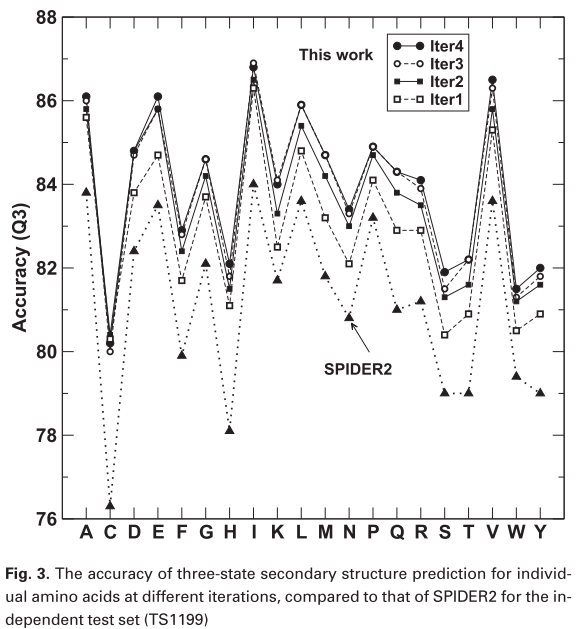
\includegraphics[width=0.7\linewidth]{peramino}
\end{figure}
\subsubsection{Matthews correlation coefficient}
"Besides Q3 and Q8, Matthews correlation coefficient (Matthews, 1975) was also used as performance metric, as it takes true and false positives and negatives into account and provides a more balanced measurement of quality network classification capability." \cite{Fang2017}
\subsubsection{Precision-recall}
\begin{figure}[h]
	\centering
	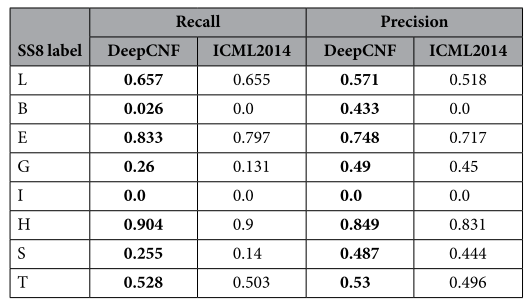
\includegraphics[width=0.7\linewidth]{prere}
	\caption{Recall and precision of DeepCNF and ICML2014 on the CB513 dataset.}
\end{figure}
\begin{figure}[h]
	\centering
	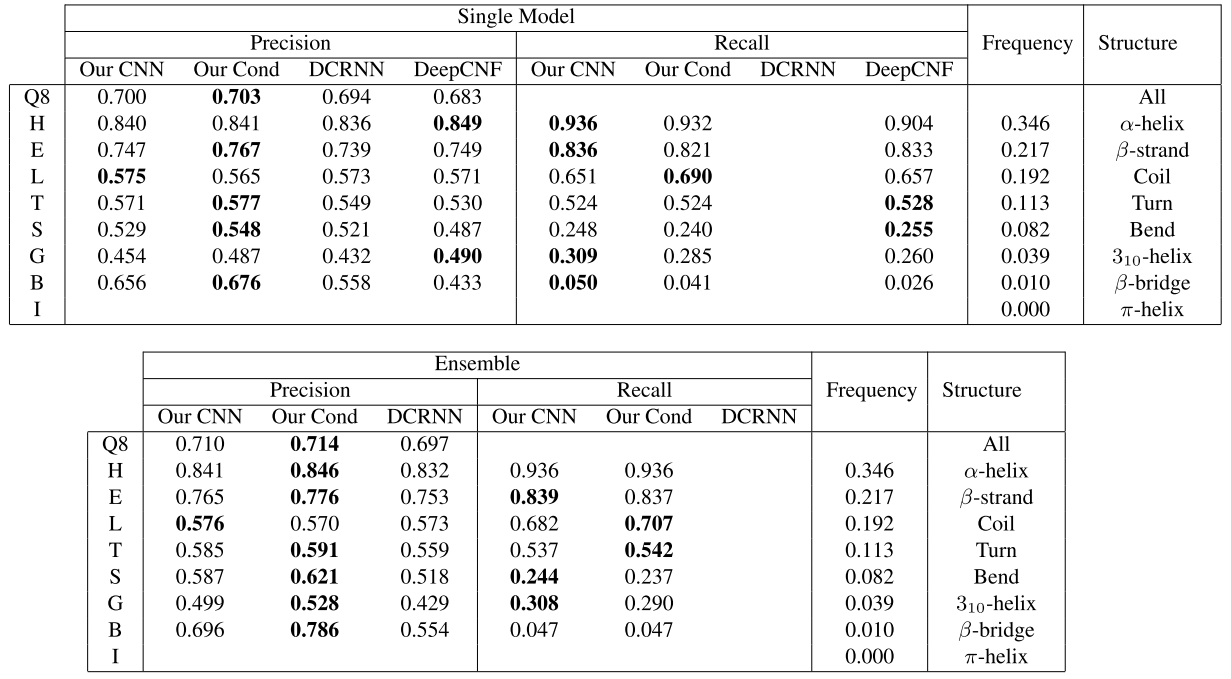
\includegraphics[width=1\linewidth]{precrec}
	\caption{Recall and precision of condCNN, DBLSTM and DeepCNF on the CB513 dataset.}
\end{figure}
\subsubsection{Confusion matrix}
\begin{figure}[h]
	\centering
	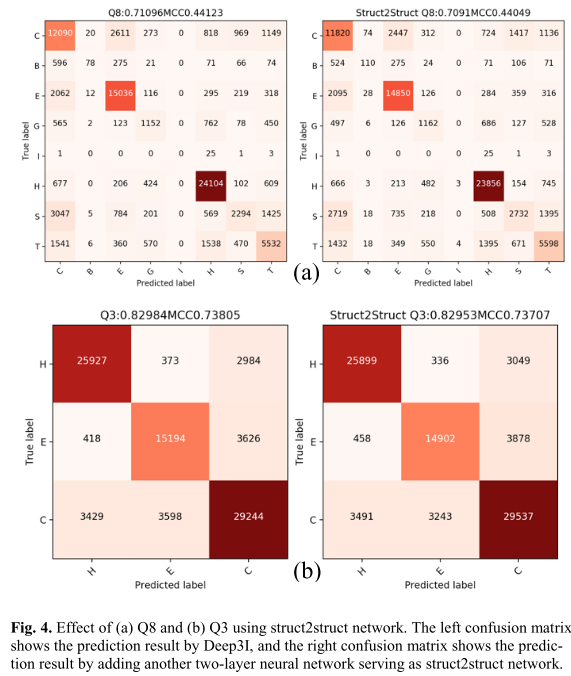
\includegraphics[width=0.7\linewidth]{confmat}
	\caption{Recall and precision of DeepCNF and ICML2014 on the CB513 dataset.}
\end{figure}
\subsubsection{ROC curve}
"Area under the receiver operating curve (AUC) (Baldi et al., 2000). To generate a receiver operating curve (ROC) one needs binary target values and continuous predictions made by the method to be evaluated. The ROC curve is then constructed by shifting the threshold for determining positive and negative predictions made by the method; each time threshold is shifted the true positive and false positive predictions are calculated and entered into a diagram with false positives on the x-axis and true positives on the y-axis. The AUC is 0.5 for a method that makes random predictions and 1 for a method that makes perfect predictions." \cite{Jurtz2017}
Per-class curves.
"A visual comparison between the gradient optimization approaches was done using a ROC (Receiver Operating Characteristics) plot, which is commonly used in decision making in Machine Learning [3] and shows the difference between methods in a clear manner. [...] In a ROC plot, the x and y axes are defined as (1 − Sp) and Se, respectively. The best prediction would be the closer to the top left corner." \cite{Hattori2017}
\subsubsection{PCC: Pearson's correlation coefficient}
"PCC calculates the correlation between the predictions made by the method and the target values. A PCC value of 1/-1 is perfect (reverse) correlation, 0 is no correlation." \cite{Jurtz2017}
\subsubsection{SOV}
"Alternatively, 3-state SS prediction could also be measured by segment of overlap (SOV) score, which can be interpreted as SS segment-based accuracy. SOV allows for small wrong predictions at SS segment ends, but penalizes more on wrong predictions in the middle region of a SS segment49. [...]
For 3-state SS prediction, we also calculate the SOV (Segment of OVerlap) score49, which measures how well the observed and the predicted SS segments match. In particular, the SOV measure assigns a lower score to the prediction deviating from observed SS segment length distribution even if it has high Q3 accuracy (i.e., per-residue accuracy)31. A wrong prediction in the middle region of a SS segment results in a lower SOV score than a wrong prediction at the terminal regions. A detailed definition of SOV is described in32, and also in our Supplemental File." \cite{Wang2016}
"The Segment Overlap score (SOV) measures overlap between the observed and the predicted secondary structure segments instead of per-residue accuracy, proposed by Zemla et. al. (Zemla, Venclovas, Fidelis, \& Rost, 1999). The predictions that have high per-residue accuracy but deviate from experimental segment length distributions have lower SOV scores (Im, 2008). SOV score ranges from 0 to 1 with 1 indicating the perfect overlap. Brief description of SOV from (Zemla, et al., 1999) is as follows. To calculate SOV, the (predicted) secondary structure of one protein sequence is parsed into segments such that each segment has a single secondary structure type. Let S1 be the observed secondary structure and S2 the predicted secondary structure. For each type ?? ∈ {??, ??, ??}, ??(??) is the set of segment pair (??1, ??2) with type ?? where s1 is from S1, s2 is from S2 and ??1 and ??2 overlap in at least one residue. That is, ??(??) = {(??1, ??2) ∶ ??1 ∩ ??2 ≠ 0 and ??1 ?????? ??2 have type ??}. In contrast, ??′(??) = {??1 ∶ ??1 ∩ ??2 = 0 and ??1 ?????? ??2 have type ??}.
Then the segment overlap score between S1 and S2 is calculated as follows.
??????(??1, ??2) =
?? ∑ 1
?? ∈ {??,??,??} ∑(??1,??2)∈??(??)
min(??1,??2)+??(??1,??2) max (??1,??2)
∙ ??(??1) (1)
where min(??1, ??2) is the length of the overlap between s1 and s2, max(??1, ??2) is the length of the total span of s1 and s2, and ??(??1) is the length of s1, ??(??1, ??2) is defined as min( max(??1, ??2) − min (??1, ??2), min(??1, ??2),
⌊
??(??2) 2 ⌋, ⌊
??(??1) 2 ⌋ ) , and ?? is defined as ∑
?? ∈ {??,??,??} ??(??) where ??(??) = ∑(??1,??2)∈??(??) ??(??1) + ∑??1∈??′(??) ??(??1)" \cite{Wang2016}
\subsubsection{P-value}
"A statistical test indicates that the advantage of DeepCNF over other methods is significant, as shown in Supplemental Table S3. The p-values in the table are calculated by pairwise student’s t-test between DeepCNF and the other methods. The smaller the p-value, the more significant the advantage of DeepCNF over others is. In summary, DeepCNF not only obtains better Q3 accuracy, but also better SOV score." \cite{Wang2016}

"The differences between this work and all other methods are statistically significant (P<0.05)." \cite{Heffernan2017}
\subsection{Hard targets}
"When only 85 CASP10 and CASP11 hard targets are evaluated [...] All the methods have lower Q3 accuracy on these hard targets than on the whole datasets since all the test methods use sequence profiles as input features and a hard target usually has sparse sequence profile that carries little evolutionary information. In addition, the hard targets do not have good structure homologs in the training set, so a predictor cannot copy SS labels from the training data as prediction" \cite{Wang2016}

\subsection{Superfamilies}
"An alternative way to select non-redundant proteins for training and test is to pick one representative from each protein superfamily defined by CATH56 or SCOP57. By using test proteins in different superfamilies than the training proteins, we can reduce the bias incurred by the sequence profile similarity between the training and test proteins. To fulfill this, we use the publically available JPRED training and test data47 (http://www.compbio. dundee.ac.uk/jpred4/about.shtml), which has 1338 training and 149 test proteins, respectively, each of which belongs to a different superfamily." \cite{Wang2016}

"Although the training and test proteins may not have similar primary sequences, their sequence profiles may be still similar, so one may wonder if our improvement is due to the sequence profile similarity between the test and training proteins. We conducted one stricter experiment to study this problem. In particular, we retrained our DeepCNF models using the 1338 JPRED training proteins and tested the resultant models on the 149 JPRED test proteins47. All the test and training proteins belong to different superfamilies. That is, it is unlikely that one test protein shares similar sequence profile with one training protein. The sequence profiles of these JPRED training and test proteins are generated from an NR database dated in 2012- 10-26. We divided the training set into 7 groups according to the JPRED cross-validation sets (available at http:// www.compbio.dundee.ac.uk/jpred4/about.shtml) and then trained 7 DeepCNF models separately. Each model is trained by the proteins in 6 groups" \cite{Wang2016}

\subsection{Class imbalance and data scarcity}
"Precision is very stable, while recall dramatically lowers according to the frequency of labels. This suggests that our model picked up on several key properties of labels with few training examples, but missed many. More training data is one way to solve this issue." \cite{Lin2016}

"with analysis according to the sensitivity, specificity and frequency of the classes, it is possible to verify that the DBLSTM approach can achieve better results if training with data augmentation is used." \cite{Hattori2017}

"We show that the architecturally simpler MUST-CNN does as well or better than more complex approaches." \cite{Lin2016}

\subsection{Neff}
"We further examine the performance of DeepCNF with respect to the amount of homologous information measured by Neff 33. The Neff of a protein measures the average number of effective amino acids across all the residues, ranging from 1 to 20 since there are only 20 amino acids in nature. A small Neff indicates that the protein has a sparse sequence profile. By contrast, a large Neff implies that the protein may have a large amount of homologous information" \cite{Wang2016}


\section{Architecture}
\subsection{CNNH\_PSS}
"As the dimension of amino acid representation is already low, we only calculate a real value for every dimension by embedding technique and don’t decrease the dimension. The residue embedding in this paper is implemented by a feedforward neural network layer before multi-scale CNN in CNNH\_PSS [42].
[...]
with the number of layers increasing, CNN model will lose the local contexts extracted by lower layers. In this paper, we propose a novel method, referred to as CNNH\_PSS, to resolve this problem. CNNH\_PSS contains a highway between any two neighbor convolutional layers in multi-scale CNN. As the number of convolutional layers increases, CNNH\_PSS can not only extract long-range inter- dependencies by higher layers, but also obtain the local contexts extracted by lower layers through highway.
[...]
In order to keep the output of convolutional layer have the same height with the input, we need to pad ⌊h/2⌋ and ⌊(h − 1)/2⌋ m-dimensional zero vectors to the head and the tail of the input x1: L, respectively, where h is the length of convolutional kernels in the convolutional layer.
[...]
In CNNH\_PSS, each convolutional layer except the last layer has three accesses to the next layer. Two accesses are used to deliver information from the current layer to the output and convolution kernels of the next layer, respectively. The other one is a weight used to determine the share of information in for information from highway. So the output ct of the tth convolutional layer is the weighted sum of the information delivered by highway from last layer and that out- putted by the convolution kernels of current layer zt ¼ δ wzct−1??
ð6Þ
ct ¼ 1−ztðÞ? ft θt ct−1 þ zt ? ct−1
ð7Þ
where δ(⋅)is sigmoid function,zt is the weight of the highway and ft θt ð?Þ is the convolution operation of current convolutional layer. So the output of the tth convolutional layer contains two portion: information from the (t−1)th convolutional layer delivered by highway and that outputted by the convolution kernels of current layer.
[...]
CNNH\_PSS achieves the best performance when the number of convolutional layers is 5.
[...]
kernel length of 11" \cite{Zhou2018}

\subsection{DeepCNF} \label{DeepCNF}
"our deep convolutional neural networks are better in predicting beta turn (T), high curvature loop (S), and irregular loop (L) states, which appear more often at the boundary of a helix or sheet segment. The other reason is that the conditional random fields in our method models the interdependency among adjacent residues in a SS segment, which helps reduce erroneous predictions in the middle region of a segment." \cite{Wang2016}

"Overall, our method obtains better recall and precision for each state, especially those non-ordinary states such as G, S and T." \cite{Wang2016}

"This result could be due to the fact that S, T, and L state may be impacted by medium-range information on the pro- tein sequence36 and our method is better than the others in modeling this kind of information." \cite{Wang2016}

Available at http://raptorx.uchicago.edu/download/.

\subsection{DCRNN}
"The embedded sequence features and the original profile features are fed into multiscale CNN layers with different kernel sizes to extract multiscale local contextual features. The concatenated multiscale local contexts flow into three stacked BGRU layers, which capture global contexts. On top of the cascaded CNN and BGRU layers, there are two fully connected hidden layers taking concatenated local and global contexts as input. The output from the second fully connected layer with softmax activation is fed into the output layer, which performs 8−category secondary structure and 4−category solvent accessibility classification." \cite{Li2016}
\begin{figure}[h]
	\centering
	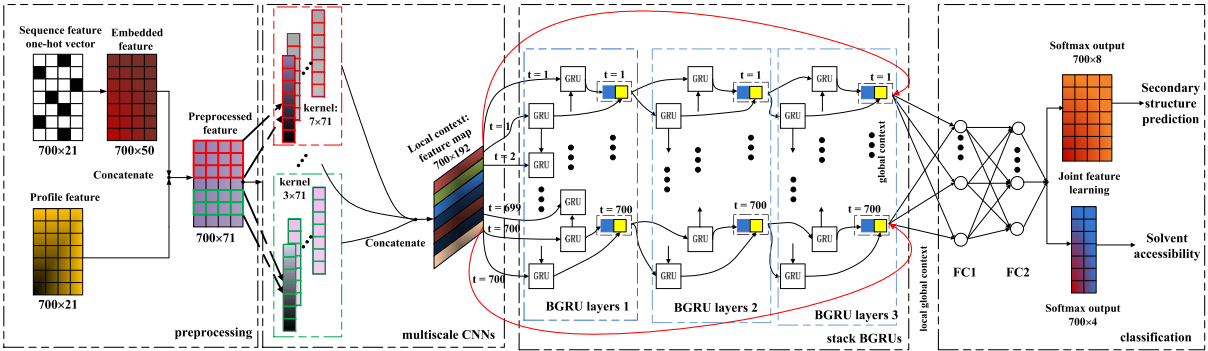
\includegraphics[width=1\linewidth]{DCRNN}
\end{figure}

"it is the first time to apply bidirectional GRU layers to secondary protein structure prediction. An ablation study indicates they form the most important component of our deep neural network." \cite{Li2016}

\subsection{MUFold-SS}
"improves upon the test accuracy of these models using different neural networks and deep architectural innovations, including residual network (He et al., 2016; He et al., 2016), inception network (Ioffe and Szegedy, 2015; Szegedy et al., 2016; Szegedy et al., 2015), batch normalization (Ioffe and Szegedy, 2015), dropout and weight constraining (Srivastava et al., 2014), etc." \cite{Fang2017}

"Several of the latest deep-learning methods on biolog- ical sequences were applied for the first time, which may provide useful information for applying these tools on other bioinformatics problems" \cite{Fang2017}

"Figure 1 shows the basic Inception (Szegedy et al., 2016) module of the Deep3I model. Since the convolutions with large spatial filters are com- putationally expensive, a hierarchical layer of convolutions with small spatial filters was used." \cite{Fang2017}
\begin{figure}[h]
	\centering
	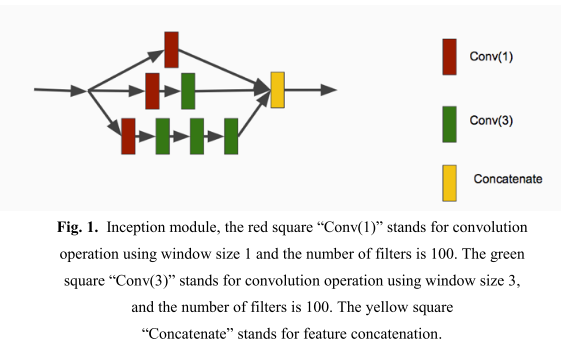
\includegraphics[width=0.7\linewidth]{inception}
\end{figure}
"Figure 2 shows how an inception-inside-inception module consists of
many inception modules. Each layer in the inception module consists of an inception unit module, as a recursion of applying the inception unit inside another inception block." \cite{Fang2017}
\begin{figure}[h]
	\centering
	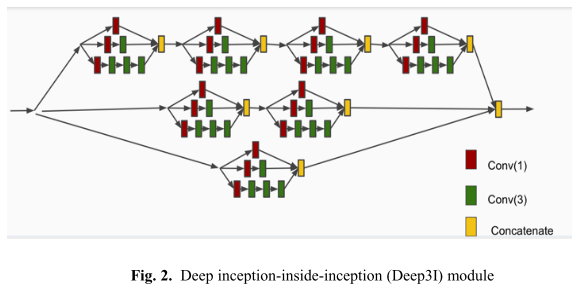
\includegraphics[width=0.7\linewidth]{IiI}
\end{figure}
"Figure 3 presents the design of Deep3I network, after many trials. Add-
ing more Deep3I blocks is possible but requires more memory and com- puting time. Other Inception (Szegety et al., 2016) blocks were explored too." \cite{Fang2017}
\begin{figure}[h]
	\centering
	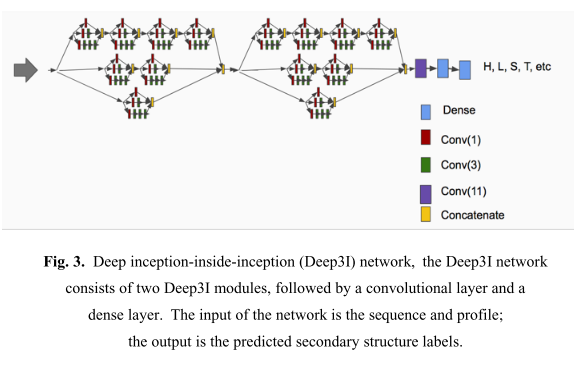
\includegraphics[width=0.7\linewidth]{Mufold}
	\label{fig:Mufold}
\end{figure}
"The proposed Deep3I network (see Fig. 2) differs from the previous net- work (Li and Yu, 2016; Busia and Jaitly, 2017) in that the latter ones used residual blocks and multi-scale layer containing CNN layers with a con- volution window size of 3, 7, and 9 to discover protein local and global context. Deep3I consists of stacked CNN layers, whose convolution win- dow size is only 3. When stacked deep convolution blocks are put to- gether, they can perform both local and global context extraction. Apply- ing convolution on top of convolution, the sliding window will cover a wide range of protein sequences by using this hierarchical convolutional operation." \cite{Fang2017}

"Each convolution layer consists of four consecutive operations: 1) The convolution operation with certain kernel size. 2) The batch nor- malization (Ioffe and Szegedy, 2015) operation is applied to help speed up
the training process and acts as a regularizer. 3) The activation operation, ‘ReLU,’ (Radford et al., 2015) was used as an activation function. 4) The dropout (Srivastava et al., 2014) operation to prevent the neural network from overfitting randomly drops neurons during the deep network training process such that the network can avoid too much co-adapting.

During implementation, the dropout rate was set to 0.4. During net-
work training, the learning rate scheduler from Keras was also used to control the learning rate. The early stopping mechanism from Keras was used to stop network training when the monitored validation quantity (such as validation loss and/or validation accuracy) stopped improving. The “patience” (i.e., the number of epochs with no improvement after which training was stopped) was set between 8 to 12 in experiments. Ten- sorBoard from Keras was used to visualize dynamic graphs of the training and validation metrics" \cite{Fang2017}

\subsection{DBLSTM}
"it is important to mention that the ReLU is used in
the input of each layer. Also, the Dropout technique is used in the output of each layer during the training task." \cite{Hattori2017}

"The cost function used in this work is the categorical cross-
entropy between the predicted (pi,j) and target (ti,j) protein secondary structure classes, as presented in Equation 8. It is the loss function (Li) for multi-class problems with softmax output.
Li = −ti,jlog(pi,j)" \cite{Hattori2017}

\begin{figure}[h]
	\centering
	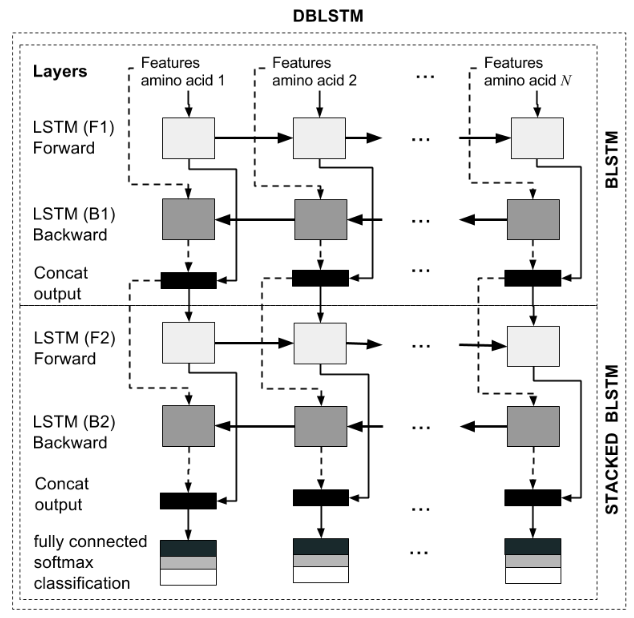
\includegraphics[width=0.7\linewidth]{DBLSTM}
	\label{fig:DBLSTM}
\end{figure}

\subsection{Jurtz}
"Convolutional filters of sizes 3, 5 and 7 neurons first processed the input. For each filter size 16 filters were used. A dense layer of 200 hidden neurons processed the output of the convolutional filters together with the original input. Batch normalization was applied to this dense layer after the linear combination and before the nonlinearity (Ioffe and Szegedy, 2015). The output of the dense layer was the input to forward and backward LSTM layers, each containing 400 LSTM memory blocks. Dropout (p=0.5) was applied to the output of the LSTM layers and they were both connected to a dense layer containing 200 hidden neurons. This dense layer fed into the output layer containing 8 neurons. An eight-way softmax function was applied to provide the secondary structure prediction according to the Q8 DSSP classes.

For the convolutional and dense layers ReLU nonlinearities were used, the LSTM followed the default implementation by (Graves, 2012).

CNN + LSTM:
Input layer,
Conv: [3x , 5x , 7x ] 16,
Batch normalization,
Dense (200),
Batch normalization + Input layer,
[Forward LSTM (400), Backward LSTM (400)],
Dropout (50\%),
Dense (200),
Secondary structure,
" \cite{Jurtz2017}
\begin{figure}
\centering
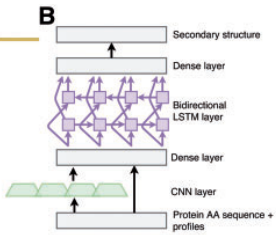
\includegraphics[width=0.5\linewidth]{jurtz}
\label{fig:jurtz}
\end{figure}

\subsection{SPIDER3}
As shown in Figure 1, the model uses two BRNN layers with 256 nodes per direction, followed by two more fully connected hidden layers with 1024 and 512 nodes, respectively. The BRNN layers use Long Short-Term Memory (LSTM) cells (Hochreiter and Schmidhuber, 1997) due to their ability to learn both distant and close intra-sequence dependencies. The fully connected nodes in the network each use Rectified Linear Unit (ReLU) activations." \cite{Heffernan2017}

\subsection{Busia}
"This model achieves 70.0\% per amino acid accuracy on the CB513 benchmark dataset without use of standard performance-boosting techniques such as ensembling or multitask learning. We then improve upon this state-of-the-art result using a novel chained prediction approach which frames the secondary structure prediction as a next-step prediction problem. This sequential model achieves 70.3\% Q8 accuracy on CB513 with a single model; an ensemble of these models produces 71.4\% Q8 accuracy on the same test set, improving upon the previous overall state of the art for the eight-class secondary structure problem." \cite{Busia2017}

"residual connections (He et al., 2015), and multi-scale convolutional filters (Szegedy et al., 2015; Szegedy, Ioffe, \& Vanhoucke, 2016). we introduce a new approach using chained models for next-step prediction of the target sequences of secondary structure la- bels (Sutskever, Vinyals, \& Le, 2014; Bengio et al., 2015; Gkioxari, Toshev, \& Jaitly, 2016). We do this by incorporating next-step conditioning into our convolutional architecture: we condition individual predictions on both local sequence data and past target labels, and control for over- fitting with scheduled sampling during training (Bengio et al., 2015)." \cite{Busia2017}

"We begin with a simplistic baseline: we feed a fixed-sized context window of seventeen amino acids (padding edge-cases with no-sequence tokens) through five fully- connected layers of 455 rectified-linear units each in order to predict the secondary structure label of the central amino acid via a softmax output layer." \cite{Busia2017}

"Designed for image detection and classification tasks, the Inception architecture (Szegedy et al., 2015; Szegedy, Ioffe, \& Vanhoucke, 2016) makes heavy use of multi-scale convolutional layers which simultaneously apply different filter sizes to compute features on several scales. Similar to this Inception model, we use blocks composed of single- and multi-scale convolutional layers as part of the larger neural network" \cite{Busia2017}

"We combine the approaches of three other successful image recognition models to develop a modified skip connection between layers of our model. The ResNET model (He et al., 2015) improved performance on image classification by introducing residual connections consisting of additive identity shortcuts between the outputs of lower layers and the inputs to higher layers to improve information flow throughout the network. Huang, Liu, \& Weinberger’s (2016) work on the DenseNet architecture provides an alternate approach to improving information flow which feeds the depth concatenation of the outputs of all previous layers in the model to any given layer. Finally, Network-in-Network architectures make use of 1x1-filter convolutions to control for high-dimensionality induced by successive multi-scale convolutions on images (Lin, Chen, \& Yan, 2013). [...] We break our model into blocks of multi- and single-scale convolutions, combining the outputs within blocks via depth concatenation. Then, similar to ResNet, we introduce connections between blocks, but find that depth concatenation of features gives vastly better training and validation performance than typical additive connections. We also make use of 1-filter convolutions to avoid an explosion in the number of features with the addition of blocks to the model. Thus, unlike previous image recognition models, our skip connections are formed by applying a 1-filter with depth 96 to condense the features learned by the layers in the previous block to a smaller fixed-number of features before concatenating those to the output of the current block. [...] Our final convolutional model in Figure 2(b) consists of two of these convolutional blocks connected by our modified skip connections, followed by two fully-connected layers of 455 units, the first of which receives a fixed-context window of eleven features produced by the final convolutional block. Each multi-scale layer contains 3-, 7-, and 9-filters of depth 64, and is followed by a single convolution with a filter size of 9 and a depth of 24." \cite{Busia2017}
\begin{figure}
	\centering
	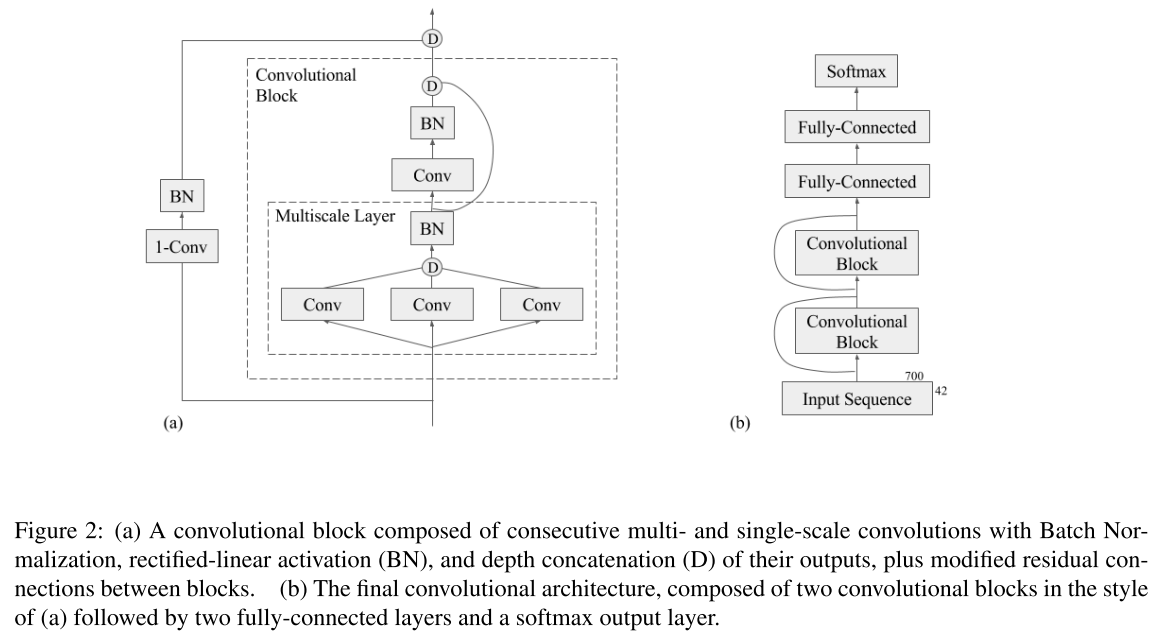
\includegraphics[width=1\linewidth]{busiacnn}
	\label{fig:busiacnn}
\end{figure}
\begin{figure}
	\centering
	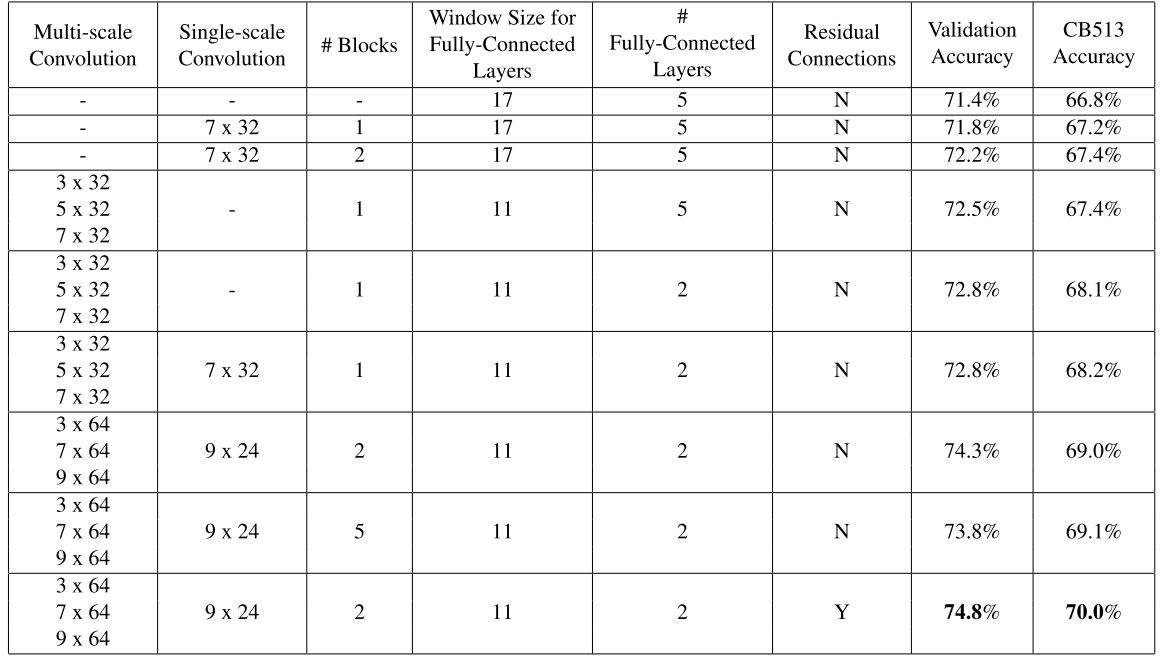
\includegraphics[width=1\linewidth]{filtersbusia}
\end{figure}
"1.0\% performance boost of adding our modified residual connections is much more impressive than the 0.1\% gained by naively adding more convolutional blocks to the model. [...] Moreover, we believe these modified residual connections improve the model’s ability to retain information about smaller local contexts within the sequence instead of allowing them to be washed out by longer-range features learned by subsequent convolutions over larger sequence patches." \cite{Busia2017}

"Here, we re-frame the protein structure prediction problem as a chained prediction task by introducing next-step conditioning, effectively using a language model over the sequences of structure labels. We model the dependencies between secondary structure labels by conditioning the current prediction on the previous structure labels in addition to the current input. This technique has led to substantial improvements in the performance of sequence- to-sequence models on complex tasks such as machine translation and pose prediction (Sutskever, Vinyals, \& Le, 2014; Bengio et al., 2015; Gkioxari, Toshev, \& Jaitly, 2016). Standard techniques for secondary structure prediction attempt to model the secondary structure y = y1, y2 · · · yL of a protein sequence of length L using its input amino acid sequence x = x1, x2, · · · xL, where yi is the secondary structure label of the amino acid at index i and xi is the amino acid at index i (or more generally, its descriptors, such as real-valued sequence information from PSSM matrices). This is typical of both convolutional and recurrent neural network approaches, which optimize a model under the following conditional distribution assumption: p (y1, · · · yL|x1 · · · xL) = p (y1|x) p (yi|x) In contrast, introducing next-step conditioning forgoes the assumption of independence between predictions and allows us to instead attempt to model the probability distribution of y1 · · · yL using a chain rule decomposition:
?L p (y1, · · · yL|x1 · · · xL) = p (y1|x) p (yi|x, y<i)
i=2
In typical applications of sequence-to-sequence modeling, this conditioning is implemented using recurrent neural network layers; here, we instead modify the approach to work as an extension of our convolutional architecture from the preceding section. We hold the convolutional architecture constant–with all hyperparameters kept as previously described–and introduce conditioning on a context of previous secondary structure labels during training by appending the input sequence (padded on the edges by no-sequence tokens) with a copy of the secondary structure labels shifted by the effective total window size W of the convolutional model (see Figure 3). Note that W depends on the architecture of the neural network and is a function of the widths of the convolutional filters and the window size that is input into the fully-connected layers. Using this approach, for a given residue in the sequence, the model will integrate information not only from the relevant surrounding amino acids, but also from the additional context provided by the previous W secondary structure labels. Thus, we effectively model p (yi|x, y<i) as p ? yi|x, y(i−W)···(i−1) ? using our multi-scale convolutional neural network.
\begin{figure}
	\centering
	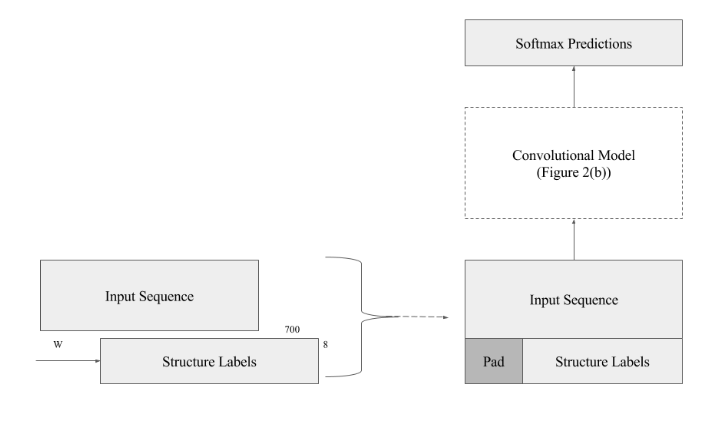
\includegraphics[width=0.8\linewidth]{conditioning}
\end{figure}
During inference, the true previous secondary structure labels are not available. Instead, we find the label sequence y that maximizes p (y1, · · · yL|x1 · · · xL) by decoding the input sequence using a standard left-to-right beam search. We use a beam search of size eight: for any given protein, we make sequential predictions and on each step maintain the eight most likely partial sequences of secondary structure assignments based on the running logarithmic probabilities produced by the model. These hypotheses are, in turn, fed as past context to the next beam search step. Additional details about this beam search procedure can be found in Sutskever, Vinyals, \& Le’s (2014) work on sequence-to-sequence modeling with neural networks.
We find that the model is able to learn to achieve fairly high accuracy at predicting the next label when the previous labels are indeed correct; however, during inference the previous labels may not be entirely accurate as they are selected from the predicted probability distribution over the eight possible secondary structure classes during beam search. This mismatch between test and train conditions hurts the performance of the model. In light of this, we make use of a simple implementation of scheduled sampling to introduce uncertainty into the previous structure labels seen as context during training to make the model more robust to past mistakes. In scheduled sampling, the model is increasingly fed its own predictions during training in place of the ground truth past labels (Bengio et al., 2015). This means we sample the structure labels which are fed as past context during training, call them c, from the model’s predictions at some rate r. Here, for a given protein, we obtain a sequence of sampled labels ˆy for each protein where ˆyi is drawn from the multinomial distribution described by p ? yi|x, ˆy(i−W)···(i−1) ? instead of p yi|x, y(i−W)···(i−1) ? ?. Then, we update c according to
ci = b · ˆyi + (1 − b) · yi where b ∼ Binomial(r). We initialize r to 40\%, and gradually increase it by 10\% every 750,000 training iterations.

In addition to evaluating single models, we also train and evaluate an ensemble of ten independently trained models for each of the convolutional and next-step conditioned models. Each individual model is trained on a randomly sampled training and validation subsets. The outputs of these ten models are combined by averaging their predicted logarithmic probabilities over the secondary structure labels. Let us denote the probability distribution predicted by the mth model in an ensemble as pm. Then, a given prediction ˆyi of an ensemble of N convolutional models is determined by evaluating pˆ =1?N log pm (yi|x) and taking ˆyi to be the secondary structure label with the highest resulting probability. For the next-step conditioned models, this ensembling process takes place sequentially during the beam search process. On the kth step of the search for a protein of length L, we calculate the average predicted logarithmic probabilities across the N models in the ensemble based on the inputs x and past context from the current hypotheses pˆ = 1N?Nlog pm yi|x, ˆy(i−W)···(i−1) ? ? for each of the eight current partial hypotheses of secondary structure sequences. We add this value to the running logarithmic probability k−1?log ˆp yi|x, ˆy(i−W)···(i−1) ? ? and determine the new eight most probable partial hypotheses from this result. The ensemble’s final predictions are obtained at the end of the beam search by selecting, out of the eight hypotheses, the sequence of secondary structure labels which has the highest probability according to the above equation at the final step k = L of the beam search process. We estimate error bars on the Q8 accuracy of these ensembles via bootstrapping: we train fifteen models total and calculate the Q8 performance metric for ten different randomly selected subsets of ten of these trained models, then estimate the standard error from the spread of the resulting values." \cite{Busia2017}

\subsection{Window size}
"We fix the window size to 11 because the average length of an alpha helix is around eleven residues58 and that of a beta strand is around six59" \cite{Wang2016}

\subsection{Adjancent labels}
"the conditional random fields in our method models the interdependency among adjacent residues in a SS segment, which helps reduce erroneous predictions in the middle region of a segment." \cite{Wang2016}

"The struct2struct network was proposed by (Rost and Sander, 1993). Adding the struct2struct network after the Deep3I network can fine-tune the predicted results as it takes into consideration the consecutive patterns. For example, an ?-helix should consist of at least three consecutive amino ac- ids. The predicted secondary structure from the Deep3I may violate such a pattern, i.e., not protein-like. By further feeding the initial predicted secondary structures into the second struct2struct network, the result will be fine-tuned and more protein-like. The input for the struct2struct network is the output from the previous Deep3I prediction, i.e., the predicted prob- ability of each class from the last Softmax layer, and the output of struct2struct network is again the secondary structure label. The traditional struct2struct network described in (Rost and Sander, 1993) used two lay- ers of simple neural networks. In this implementation, two layers of convolutional layers were used and the convolution window size was 11. The added struct2struct network may not improve the Q3(Q8) much, but it can make the prediction more protein like and help predict some small classes like B, G, S, T." \cite{Fang2017}

"Besides that, a struct2struct (Rost and Sander, 1993) network is added after Deep3I for fine-tuning the secondary structure prediction. This network acts as a fine-tuning layer on top of Deep3I and can further make the prediction results more protein-like." \cite{Fang2017}

"The struct2struct network improved the Q3(Q8) performance but not that significantly. Since the most improvement can be achieved by the Deep3I network, the struct2struct can act as a refinement layer (See Fig. 4a for Q8 and Fig. 4b for Q3). Nevertheless, it correctly predicted more small classes like B, G, S and T for Q8." \cite{Fang2017}

"Here, we re-frame the protein structure prediction problem as a chained prediction task by introducing next-step conditioning, effectively using a language model over the sequences of structure labels. We model the dependencies between secondary structure labels by conditioning the current prediction on the previous structure labels in addition to the current input. This technique has led to substantial improvements in the performance of sequence- to-sequence models on complex tasks such as machine translation and pose prediction (Sutskever, Vinyals, \& Le, 2014; Bengio et al., 2015; Gkioxari, Toshev, \& Jaitly, 2016). Standard techniques for secondary structure prediction attempt to model the secondary structure y = y1, y2 · · · yL of a protein sequence of length L using its input amino acid sequence x = x1, x2, · · · xL, where yi is the secondary structure label of the amino acid at index i and xi is the amino acid at index i (or more generally, its descriptors, such as real-valued sequence information from PSSM matrices). This is typical of both convolutional and recurrent neural network approaches, which optimize a model under the following conditional distribution assumption: p (y1, · · · yL|x1 · · · xL) = p (y1|x) p (yi|x) In contrast, introducing next-step conditioning forgoes the assumption of independence between predictions and allows us to instead attempt to model the probability distribution of y1 · · · yL using a chain rule decomposition:
?L p (y1, · · · yL|x1 · · · xL) = p (y1|x) p (yi|x, y<i)
i=2
In typical applications of sequence-to-sequence modeling, this conditioning is implemented using recurrent neural network layers; here, we instead modify the approach to work as an extension of our convolutional architecture from the preceding section. We hold the convolutional architecture constant–with all hyperparameters kept as previously described–and introduce conditioning on a context of previous secondary structure labels during training by appending the input sequence (padded on the edges by no-sequence tokens) with a copy of the secondary structure labels shifted by the effective total window size W of the convolutional model (see Figure 3). Note that W depends on the architecture of the neural network and is a function of the widths of the convolutional filters and the window size that is input into the fully-connected layers. Using this approach, for a given residue in the sequence, the model will integrate information not only from the relevant surrounding amino acids, but also from the additional context provided by the previous W secondary structure labels. Thus, we effectively model p (yi|x, y<i) as p ? yi|x, y(i−W)···(i−1) ? using our multi-scale convolutional neural network.
\begin{figure}
	\centering
	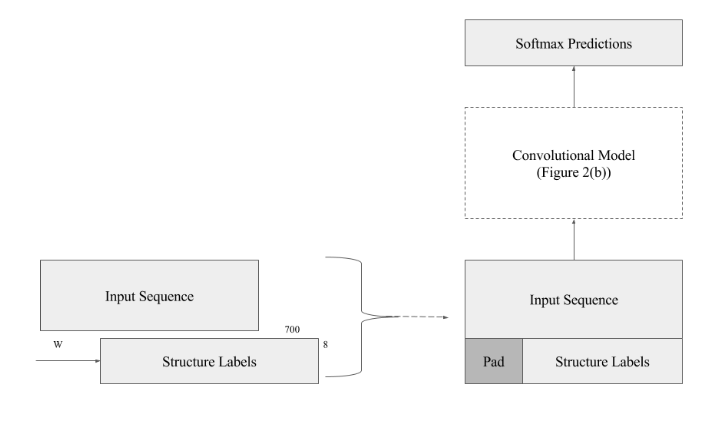
\includegraphics[width=0.8\linewidth]{conditioning}
	\label{fig:conditioning}
\end{figure}
During inference, the true previous secondary structure labels are not available. Instead, we find the label sequence y that maximizes p (y1, · · · yL|x1 · · · xL) by decoding the input sequence using a standard left-to-right beam search. We use a beam search of size eight: for any given protein, we make sequential predictions and on each step maintain the eight most likely partial sequences of secondary structure assignments based on the running logarithmic probabilities produced by the model. These hypotheses are, in turn, fed as past context to the next beam search step. Additional details about this beam search procedure can be found in Sutskever, Vinyals, \& Le’s (2014) work on sequence-to-sequence modeling with neural networks.
We find that the model is able to learn to achieve fairly high accuracy at predicting the next label when the previous labels are indeed correct; however, during inference the previous labels may not be entirely accurate as they are selected from the predicted probability distribution over the eight possible secondary structure classes during beam search. This mismatch between test and train conditions hurts the performance of the model. In light of this, we make use of a simple implementation of scheduled sampling to introduce uncertainty into the previous structure labels seen as context during training to make the model more robust to past mistakes. In scheduled sampling, the model is increasingly fed its own predictions during training in place of the ground truth past labels (Bengio et al., 2015). This means we sample the structure labels which are fed as past context during training, call them c, from the model’s predictions at some rate r. Here, for a given protein, we obtain a sequence of sampled labels ˆy for each protein where ˆyi is drawn from the multinomial distribution described by p ? yi|x, ˆy(i−W)···(i−1) ? instead of p yi|x, y(i−W)···(i−1) ? ?. Then, we update c according to
ci = b · ˆyi + (1 − b) · yi where b ∼ Binomial(r). We initialize r to 40\%, and gradually increase it by 10\% every 750,000 training iterations." \cite{Busia2017}

"Our first attempt to train a next-step conditioned model–without scheduled sampling–was able to reach a Q8 accuracy of roughly 82\% on the validation set and 77\% on CB513 when the ground truth secondary structure labels were fed as past context, but under true inference with beam search these measures reduced to 71.9\% and 67.1\%, respectively. This large differential suggests that such an unstructured approach to conditioning on the past induces significant overfitting for protein secondary structure pre- diction; we posit that, without the relative robustness induced by scheduled sampling, this conditional model learns to almost always simply copy the previously seen label assignment during training, making it perform well on next-step prediction with ground truth labels but relatively poorly on inference when the true sequence of structure labels is not known. It is likely that the lack of assumptions regarding the nature of dependence between structure labels and the repetitive nature of secondary structure sequences combine to cause the model to “over-learn” dependencies between consecutive labels The use of scheduled sampling helps mitigate this: adding next-step conditioning to our convolutional model via a simple scheduled sampling approach improves its performance on the eight-class secondary structure problem by 0.3\%. We hypothesize, however, that some of this “over-learning” effect persists, and in particular that the recall metrics for individual classes in Table 4–especially those which are rare or tend to occur in shorter runs– suffer slightly from this copying tendency. We highlight here that the currently reported performance metrics for the next-step conditioned model are obtained without re- tuning of any architectural or regularization hyperparameters; it is likely that adjusting the amount of regularization in combination with more sophisticated sampling schedules will further widen the gap in performance between the convolutional and next-step conditioned models." \cite{Busia2017}

\section{Training}
"TensorBoard from Keras was used to visualize dynamic graphs of the training and validation metrics." \cite{Fang2017}

\subsection{Regularization}
"Regularization techniques aim to prevent overfitting and are especially relevant for large models containing many parameters." \cite{Jurtz2017}

"Further gradient clipping (cut at norm= 20) and L2 regularization (0.0001) were used to stabilize training." \cite{Jurtz2017}
\subsubsection{Dropout}
"Dropout (Hinton et al., 2012) reduces overfitting by introducing discrete noise during training. For every training input the output of each hidden unit is set to zero with a certain preselected probability." \cite{Jurtz2017}

"Dropout (p=0.5) was applied to the output of the LSTM layers" \cite{Jurtz2017}

"the dropout rate was set to 0.4." \cite{Fang2017}

"To reduce network overfitting, we utilize the dropout algorithm (Srivastava et al., 2014) with a dropout ratio of 50\% during training." \cite{Heffernan2017}

"We follow a typical dropout approach: 20\% of the units in each layer (and their connections) are randomly dropped from the neural network during training, and at test time the full network is used with the weights scaled by the dropout factor of 20\%. [...] introducing batch normalization just prior to the application of a rectified-linear non-linearity followed by 40\% dropout provides a strong boost in validation accuracy. The fully-connected layers, however, instead maintain a max-norm constraint of 0.150 on the l2-norm of their weights." \cite{Busia2017}
\subsubsection{Batch Normalization}
"Batch normalization (Ioffe and Szegedy, 2015) re-parameterizes the hidden unit activation in order to increase convergence speed but also makes the output stochastic, creating a regularizing effect." \cite{Jurtz2017}

"Batch normalization was applied to this dense layer after the linear combination and before the nonlinearity (Ioffe and Szegedy, 2015)." \cite{Jurtz2017}

"Batch Normalization is a technique for mitigating underfitting by normalizing layer inputs within the neural network architecture according to mini-batch statistics to reduce the shift in each layer’s input distribution as the model trains (Ioffe \& Szegedy, 2015). This has been shown to accelerate training on image recognition tasks, and we find that, for our problem, introducing batch normalization just prior to the application of a rectified-linear non-linearity followed by 40\% dropout provides a strong boost in validation accuracy. The fully-connected layers, however, instead maintain a max-norm constraint of 0.150 on the l2-norm of their weights." \cite{Busia2017}

\subsection{Cost function}
"The network was trained by calculating the cross entropy for each secondary protein structure prediction," \cite{Jurtz2017}

"For the secondary structure prediction the network uses the cross-entropy loss function which is well suited to classification problems (LeCun et al., 2006). [...] During training both of these networks mask out the loss contributed by any undefined labels, such as residues with no secondary structure assignment according to the program Dictionary of Secondary Structure of Proteins (DSSP) (Kabsch and Sander 1983)." \cite{Heffernan2017}

"We train these model parameters using TensorFlow’s implementation of the cross-entropy loss (masking out padded sequence locations with zeros)" \cite{Busia2017}
\subsection{Epochs and batch size}
"Each of these networks was trained for a total of 150 epochs using a mini-batch size of 64 (shuffling the training examples after each epoch)" \cite{Jurtz2017}

"During training, we use a randomly selected mini-batch of 50 protein sequences on each iteration, where a single protein sequence has an average length of roughly 214 amino acid residues." \cite{Busia2017}

\subsection{Early stopping}
"The early stopping mechanism from Keras was used to stop network training when the monitored validation quantity (such as validation loss and/or validation accuracy) stopped improving. The “patience” (i.e., the number of epochs with no improvement after which training was stopped) was set between 8 to 12 in experiments." \cite{Fang2017}

"the validation set was used to pick the weights from the best performing epoch" \cite{Jurtz2017}

"The validation set loss was used for early stopping during training to stop the networks from overfitting to the training" \cite{Heffernan2017}

"enforce early-stopping based on Q8 accuracy on the held-out validation set." \cite{Busia2017}

\subsection{Weight initialization and norm constraint}
\subsubsection{Weight initialization}
"The convolutional and dense layers had their weights initialized with glorot uniform (Glorot and Bengio, 2010) (while the LSTM was initialized with a gaussian random (mean=0, std=0.1)). All biases where initalized to zero." \cite{Jurtz2017}

"In all cases, biases in the model are initialized to 0.1; model weights are randomly initialized according to a zero-centered Gaus- sian distribution with a standard deviation of3.0/√ I where I is the number of inputs into the layer." \cite{Busia2017}
\subsubsection{Weight norm constraint}
"We apply a combination of dropout and max-norm constraint on the model weights–this has been shown to give notable performance improvements even when the number of model parameters drastically outnumbers the size of the dataset (Srivastava et al., 2014). [...] Max-norm constraint, on the other hand, rescales model weights as necessary to force the l2-norm of every unit’s incoming weights to be at most a specified value (Srivastava et al., 2014); we find significant improvements from adding a weight-norm constraint of 0.04614. [...] The fully-connected layers, however, instead maintain a max-norm constraint of 0.150 on the l2-norm of their weights." \cite{Busia2017}

\subsection{Cross-validation}
"we randomly divide the training set (containing 5600 CullPDB proteins) into 5 subsets and then use 4 subsets as training and one as validation." \cite{Wang2016}

"We will determine the regularization factor by cross-validation." \cite{Wang2016}

"We divided the training set into 7 groups according to the JPRED cross-validation sets (available at http:// www.compbio.dundee.ac.uk/jpred4/about.shtml) and then trained 7 DeepCNF models separately. Each model is trained by the proteins in 6 groups" \cite{Wang2016}

"Before applying regularization techniques it is important to partition the dataset carefully dealing with data redundancy and set up the neural network training using cross-validation. For training and performance evaluation of neural networks, a training set on which the model parameters are trained by forward- and backpropagation, a validation set for early stopping (i.e. training is stopped when the best performance is reached on this dataset to avoid overfitting to the training data) and a test set for independent evaluation of the model performance, are normally used. To ensure optimal model training and reliable model evaluation, it is essential that limited data redundancy is present between these three data sets. What defines redundancy however depends strongly on type of data at hand, and most often is based on expert knowledge about the given biological problem. Failing to deal with data redundancy will most often lead to either poorly trained (i.e. overfitted) models, and/or overestimation of model performance. With this in mind, five fold nested cross-validation is often used to train machine learning models. The original dataset is split into five partitions (in a manner properly dealing with data redundancy). In turn, each of these five partitions are left out for testing, the remaining partitions are used to train 4 models each using 3 partitions for training and one for validation, and the test set is evaluated against this ensemble of 4 models. A variant of nested cross-validation, is simple cross-validation where the validation set is omitted, the model is trained excluding early stopping on 4 data partitions, and the left out test set is evaluated on this single model." \cite{Jurtz2017}

"The filtered training data were split into a training set (5278 sequences) and validation set (256 sequences)." \cite{Jurtz2017}

"The TR4590 set is also split into 10 evenly sized folds for 10-fold cross validation, each of these folds also has designated train and validation sequences. [...] For 10-fold cross validation, a full model (iteration 1–4) is trained for each fold. 10-fold validation results that are reported are the mean across each of the 10-folds." \cite{Heffernan2017}

\subsection{Gradient optimization and learning rate}
"Gradient optimization approaches are used in order to optimize the gradient descendent of the network and to control the value of the learning rate (η) which, in turn, determines the size of the steps that are taken towards the minimum error based on the cost function (See Section IV-A). In other words, η defines the velocity at which the network reach the minimum during the training process. In this work, the following approaches were evaluated: Stocastic Gradient Descendet (SGD) [28], Momentum [29], AdaGrad [30], RmsProp [31], AdaDelta [32] and Adam [33]." \cite{Hattori2017}

"There is no specific procedure for adjusting parameters of the gradient optimization approaches. In this work, we decided to use the default values for the parameters that are available in the Lasagne Framework." \cite{Hattori2017}

"the results strongly suggests that the RmsProp is the top gradient optimizer for the problem" \cite{Hattori2017}

"using the loss to subsequently update the weights with RMSProp (Hinton et al.) with a learning rate of 0.005." \cite{Jurtz2017}

"the learning rate scheduler from Keras was also used to control the learning rate." \cite{Fang2017}

"The model was trained using Adam optimization (Kingma and Ba, 2014), a method for efficient stochastic optimization that is able to compute adaptive learning rates and requires little hyper-parameter tuning" \cite{Heffernan2017}

First model:
"The model is trained using a learning rate of 0.0004–which is reduced by 50\% every 35,000 training iterations." \cite{Busia2017}
Last model:
"During training, we initialize the learning rate to 3.357e−4, and reduce it by 60\% every 200,000 training iterations." \cite{Busia2017}

"TensorFlow’s ADAM optimizer (Kingma \& Ba, 2014) with default beta and epsilon parameters. \cite{Busia2017}

\subsection{Ensemble}
"Combining ensembles of 5–10 models initialized with different random seeds usually leads to a substantial increase in performance. [...] An ensemble of 10 networks was trained by varying the seed from 1-10. [...] The final prediction of the ensemble was calculated by averaging the predictions of the 10 networks." \cite{Jurtz2017}

"In addition to evaluating single models, we also train and evaluate an ensemble of ten independently trained models for each of the convolutional and next-step conditioned models. Each individual model is trained on a randomly sampled training and validation subsets. The outputs of these ten models are combined by averaging their predicted logarithmic probabilities over the secondary structure labels. Let us denote the probability distribution predicted by the mth model in an ensemble as pm. Then, a given prediction ˆyi of an ensemble of N convolutional models is determined by evaluating pˆ =1?N log pm (yi|x) and taking ˆyi to be the secondary structure label with the highest resulting probability. For the next-step conditioned models, this ensembling process takes place sequentially during the beam search process. On the kth step of the search for a protein of length L, we calculate the average predicted logarithmic probabilities across the N models in the ensemble based on the inputs x and past context from the current hypotheses pˆ = 1N?Nlog pm yi|x, ˆy(i−W)···(i−1) ? ? for each of the eight current partial hypotheses of secondary structure sequences. We add this value to the running logarithmic probability k−1?log ˆp yi|x, ˆy(i−W)···(i−1) ? ? and determine the new eight most probable partial hypotheses from this result. The ensemble’s final predictions are obtained at the end of the beam search by selecting, out of the eight hypotheses, the sequence of secondary structure labels which has the highest probability according to the above equation at the final step k = L of the beam search process. We estimate error bars on the Q8 accuracy of these ensembles via bootstrapping: we train fifteen models total and calculate the Q8 performance metric for ten different randomly selected subsets of ten of these trained models, then estimate the standard error from the spread of the resulting values." \cite{Busia2017}

\subsection{Hardware}
"Intel Core i7 processor at 3.30GHz, a GPU Nvidia Titan X and a minimal installation of Ubuntu 14.04 LTS 2." \cite{Hattori2017}

"Parallel processing with GPUs is also essential to allow us to obtain high quality results in a reasonable computing time. As the size of the proteins and the network increase, the computational complexity will increase" \cite{Hattori2017}

"Neural network training was performed on Nvidia Tesla K40 GPUs and Nvidia Titan X GPUs." \cite{Jurtz2017}

"To speed up training, we use the GPU version of TensorFlow and train on an Nvidia GeForce Titan X GPU." \cite{Heffernan2017}

"we use asynchronous distributed training across five machines with NVIDIA Tesla K20 GPU Accelerators" \cite{Busia2017}

\subsection{Multitask learning}
"After the initial multitask model is trained, we take the top layers and each task-specific subclassifier and fine-tune the models by initializing their weights at the weights learned by the multitask model and training only on each specific task with 1/10 of the original learning rate." \cite{Lin2016}

"our current results could be further improved by the addition of multitask learning." \cite{Busia2017}


\section{Previous work}
\subsection{Initial research}
"Protein SS prediction has been extensively studied10–12,19–35. Many computational methods have been developed to predict both 3-state SS and a few to predict 8-state SS. Meanwhile, 8-state prediction may provide more detailed local structure information33,34,36. Holley \& Karplus19 and Qian \& Sejnowski20 may be the first that used neural networks (NN) to predict SS, which have been followed by a few others19,21,23,24,37. The most significant improvement in SS prediction was achieved by Rost \& Sander23 and Zvelebil et al.35 by making use of sequence profile derived from multiple sequence alignment38–40. Jones et al.24 developed a 2-stage neural network method PSIPRED, which takes PSI-BLAST sequence profile41 as input and obtains ~80\% accuracy for 3-state SS predic- tion. Other machine learning methods include bidirectional recurrent neural networks26,34,37 (which can capture spatial dependency), probabilistic graphical models25,29,42, support vector machines27,28,30,43 and hidden Markov models22,31." \cite{Wang2016}

"In the 1980s, the Q3 accuracy was below 60\% due to the lack of input features. In the 1990s, the Q3 accuracy reached above 70\% because of using the protein evolutionary information in the form of position-specific score matrices. Since then, the Q3 accu- racy has gradually improved to above 80\%." \cite{Fang2017}

"there is no consensus about the classification task which can be done using different properties of proteins. For instance, early approaches were based on stereochemical principles [12], statistics [13] and Position-specific Scoring Matrices (PSSM) [14]. More recently, [3] used the Kyte and Doolittle (K \& D) hydrophobicity scale in order to represent the aminoacids of proteins. From the approach point of view, [3] present the application and comparison of Machine Learning and Evolutionary Com- putation methods to define suitable classifiers for predicting the secondary structure of proteins, such as Gene expression programming (GEP), Sequential Minimal Optimization algo- rithm (SMO) and RandomForest (collection of tree-structured classifiers). [15]" \cite{Hattori2017}

"The accuracy of predicting protein local and global structural properties such as secondary structure and solvent accessible surface area has been stagnant for many years because of the challenge of accounting for non-local interactions between amino acid residues that are close in three-dimensional structural space but far from each other in their sequence positions. All existing machine-learning techniques relied on a sliding window of 10–20 amino acid residues to capture some ‘short to intermediate’ non-local interactions. [...] Commonly used simple Artificial Neural Networks (ANNs) (Faraggi et al., 2012), and Deep Neural Networks (DNNs) (Lyons et al., 2014; Heffernan et al., 2016, 2015), relied on their input windows of neighbouring residue infor- mation, which means that they are unable to fully learn the relation- ship between the residues in the whole sequence." \cite{Heffernan2017}

"Applications of machine learning to the protein secondary structure problem have a rich history: the use of neural networks for secondary structure prediction was pioneered by Qian and Sejnowski in 1988," \cite{Busia2017}

"The study of protein secondary structure prediction dates back to 1970s. In the 1970s, statistical models were frequently used to analyze the probability of specific amino acids appearing in different secondary structure elements [Chou and Fasman, 1974]. The Q3 accuracy, i.e., the accuracy of three-category classification: helix (H), strand (E) and coil (C), of these models was lower than 60\% due to inadequate features. In the 1990s, significant improvements were achieved by exploiting the evolutionary information of proteins from the same structural family [Rost and Sander, 1993] and position-specific scoring matrices [Jones, 1999]. During this period, the Q3 accuracy exceeded 70\% by taking advantage of these features. However, progress stalled when it came to the more challenging 8-category classification problem, which needs to distinguish among the following 8 categories of secondary structure elements: 310−helix (G), α−helix (H), π−helix (I), β−strand (E), β−bridge (B), β−turn (T), bend (S) and loop or irregular (L) [Zhou and Troyanskaya, 2014; Yaseen and Li, 2014]." \cite{Li2016}

\subsection{Recently}
"Zhou \& Troyanskaya36 reported another deep learning approach to 8-state SS prediction using a supervised generative stochastic network, which to our best knowledge may be the best 8-state predictor. However, neither Cheng nor Zhou reported a better than 80\% accuracy for 3-state prediction. SS prediction is usually evaluated by Q3 or Q8 accuracy, which measures the percent of residues for which 3-state or 8-state secondary structure is correctly predicted44. So far the best Q3 accuracy for ab initio prediction (i.e., templates are not allowed) is ~80\% obtained by PSIPRED and a few other state-of-the-art approaches such as JPRED47,48" \cite{Wang2016}

"In the 21-st century, various machine learning methods, especially artificial neural networks, have been utilized to improve the performance, e.g., SVMs [Sujun and Zhirong, 2001], recurrent neural networks (RNNs) [Pollastri et al., 2002], probabilistic graphical models such as conditional neural fields combining CRFs with neural networks [Wang et al., 2011], generative stochastic networks [Zhou and Troyanskaya, 2014]." \cite{Li2016}

\subsection{Hall of fame}
\begin{table}[h]
	\begin{tabular}{cccccc}
		\textbf{Names} & \textbf{Q3} & \textbf{Q8} & \textbf{Architecture} & \textbf{Date} & \textbf{Database} \\
		SPINE-X & 78.9\% & & & & CB513 \\
		PSIPRED & 79.2\% & & & 2000 & CB513 \\ 
		Qi		& 81.7\% &  & Multitask & 2012 &  \\ 
		\cite{Magnan2014}\footnote{As reported by \cite{Wang2016}}			& 		  90.7\% & 89.9\%	& SSPro(w template) & 2014 & CB513 \\
		JPRED 	& 81.7\% &  & 2-layer MLP & 2015 &  \\ \hline
		
		Wang 			&  	& 64.9\% 	& CNF 			& 2011 	&  \\ 
		\cite{Zhou2014}	&  	& 66.4\% 	& CGSN 			& 2014 	& CB513 \\ 
		\cite{Magnan2014}\footnote{As reported by \cite{Fang2017}} 			& 				78.6\% & 66.5\% & SSPro ab initio & 2014 & CB513\\
		\cite{Sønderby2014}	&  	& 67.45\% 	& LSTM 			& 2014 	& CB513 \\ 
		\cite{Wang2016} & 82.3\% & 68.3\% & DeepCNF 	& Jan2016 & CB513\\ 
		\cite{Lin2016} 	&  	& 68.4\% 	& MUST-CNN 		& May2016 & CB513 \\
		\cite{Li2016}	&  	& 69.7\% 	& DCRNN 		& 2016 	& CB513 \\
		\cite{Busia2017}&	& 71.4\%& Deep3I+conditioning& Feb2017 & CB513\\
		\cite{Heffernan2017} &84\% &  & SPIDER3 (LSTM) & Apr2017 & TS1199 \\
		\cite{Hattori2017} & & 68.0\%	& DBLSTM		& May2017 & CB513 \\
		\cite{Jurtz2017} &  & 70.2\%	& LSTM+CNN 		& Aug2017 & CB513 \\
		\cite{Johansen2017} & & 70.9\% & BGRU-CRF & Aug2017 & CB513\\
		\cite{Fang2017}&82.8\%& 71.05\% & MUFold-SS (Deep3I)&2017& CB513 \\
		\hline 
	
		Mine 	&  & 64.2\% & Base & 2018 &  \\ 
		Mine 	&  & 64.9\% & +struct2struct & 2018 &  \\ 
		Mine 	&  & 65.2\% & +denselayers & 2018 &  \\ 
		Mine 	&  & 67.7\% & 3-layers ResNet & 2018 &  \\ 
	\end{tabular}
	\caption{Hall of fame}
\end{table}
"CNF is the best among other methods for high frequency classes (H, E and L), considering the overall accuracy. On the other hand, it performs very poorly for low frequency classes (T, S, G, B and I)." \cite{Hattori2017}
\begin{table}[h]
	\begin{tabular}{cccc}
		\textbf{Names} & \textbf{Q8} & \textbf{Architecture} & \textbf{Date} \\
		$[$Wang et al., 2011$]$	& 64.9\% 	& CNF 			& 2011 \\ 
		\cite{Zhou2014}	& 66.4\% 	& \textbf{CGSN} 			& 2014 \\ 
		\cite{Magnan2014} & 66.5\% & SSPro (BRNN) & 2014 \\
		\cite{Sønderby2014}	& 67.45\% 	& LSTM 			& 2014 	\\ 
		\cite{Wang2016} & 68.3\% & \textbf{DeepCNF} 	& Jan 2016 \\ 
		\cite{Li2016}	& 69.7\% 	& \textbf{DCRNN} 		& Apr 2016 \\
		\cite{Lin2016} 	& 68.4\% 	& \textbf{MUST-CNN} 		& May 2016 \\
		\cite{Busia2017}& 71.4\%& \textbf{Deep3I+conditioning}& Feb 2017 \\
		\cite{Hattori2017} & 68.0\%	& DBLSTM		& May 2017 \\
		\cite{Jurtz2017} & 70.2\%	& \textbf{LSTM+CNN} 		& Aug 2017 \\
		\cite{Johansen2017} & 70.9\% & BGRU-CRF & Aug 2017 \\
		\cite{8371925} & 71.1\% & \textbf{DeepNRN} & Nov 2017 \\
		\cite{Zhou2018} & 70.3\% & \textbf{CNN+highway} & Jan 2018 \\
		\cite{Fang2017}& 70.63\% & \textbf{MUFold-SS (Deep3I)}&Feb 2018\\
	\end{tabular}
\end{table}

\section{Side problems}
\subsection{Disorder regions}
DeepCNF \cite{Wang2016},
MUFold-SS \cite{Fang2017}
"[LSTM to] protein intrinsic disorder prediction (Hanson et al., 2017)." \cite{Heffernan2017}

\subsection{Solvent accessibility}
DeepCNF \cite{Wang2016},
Jpred 90\%,
Qi,
MUST-CNN \cite{Lin2016},
MUFold-SS \cite{Fang2017}
"this could be used for other protein sequence problems–such as solvent accessibility, contact number" \cite{Busia2017}

"multi- task learning is utilized to predict secondary structure labels and amino-acid solvent accessibility simultaneously." \cite{Li2016}

"Along with the previously mentioned local structure descriptors,
a range of global solvent exposure descriptors are also important for understanding and predicting protein structure, function and inter-actions (Gilis and Rooman, 1997; Lee and Richards, 1971; Rost and Sander, 1994; Tuncbag et al., 2009). These include solvent Accessible Surface Area (ASA), Contact Number (CN) and Half Sphere Exposure (HSE). CN is a count of the number of neighbouring residues in three-dimensional space, within a specific distance cut off. HSE extends the ideas of CN and adds directionality information by differentiating between the counts in a top and bottom half of the sphere (Hamelryck, 2005).

Earlier methods for ASA prediction were limited to the prediction of discrete states (Holbrook et al., 1990; Rost and Sander, 1994; Pollastri et al., 2002b) and have since progressed to continuous value predictions (Dor and Zhou, 2007; Garg et al., 2005; Yuan and Huang, 2004; Ahmad et al., 2003; Adamczak et al., 2004; Heffernan et al., 2015). A number of methods for CN and HSE pre- diction have also been developed (Kinjo and Nishikawa, 2006; Song et al., 2008; Heffernan et al., 2016) The" \cite{Heffernan2017}

"The ASA, /, w, h, s, HSE and CN prediction network uses square loss which is well suited to regression problems (LeCun et al., 2006)." \cite{Heffernan2017}

"the first for ASA; [...] four for HSEa-up, HSEa-down, HSEb-up, and HSEb-down; and the final output node is for CN."

"The Pearson Correlation Coefficient (PCC) and Mean Absolute Error (MAE) between true and predicted values are used as the accuracy measures for ASA (Faraggi et al., 2012), HSE (Song et al., 2008) and CN (Yuan, 2005; Heffernan et al., 2016)." \cite{Heffernan2017}

"the correlation coefficient between predicted and actual solvent accessible surface areas to reach 0.80" \cite{Heffernan2017}

\subsection{Sub-cellular location}
"The dataset of 5,959 proteins with 11 possible locations (cytoplasm, nucleus, extracellular, mitochondria, plasma membrane, ER, chloroplast, Golgi apparatus, lysosome and peroxisome) created by (Höglund et al., 2006) available at the website of the University of Tübingen (https://abi.inf.uni-tuebingen.de/Services/MultiLoc/multiloc\_dataset) was used to train models to predict subcellular localization. The dataset is homology reduced to 80\% identity. 20\% of the data were held out to evaluate test performance and the rest of the data were used for training. Protein sequences longer than 1000 amino acids were truncated by removing amino acids from the middle of the sequence.

Protein sequences were encoded using profiles (constructed using PROFILpro (available at http://download.igb.uci.edu/\#sspro) with 3 blastpgp iterations against the 2016\_04 release of Uniref50 (Magnan and Baldi, 2014).

The protein sequence was first processed by a convolutional layer containing filters of sizes of 1,3,5,9,15 and 21 amino acids with 10 filters of each size. The convolutional layer was processed by a bidirectional LSTM layer with 256 LSTM memory blocks in each, the forwards and backwards layer. The activations of the hidden neurons were concatenated and fed into the attention function, representing the importance of each position in the protein sequence in regards to subcellular localization. Subsequently the weighted sum over the individual sequence positions was calculated, resulting in an attention context vector of 256 hidden neurons. The attention context vector obtained was passed to a dense layer with 512 hidden neurons that is connected to the output. This output layer contained 10 neurons, one for each possible subcellular location. ReLU nonlinearities were applied to the convolutional and dense layers and the hyperbolic tangent to the LSTM layer, a multiway softmax function was applied to the output to obtain the prediction of the subcellular localization.

All weights were initialized using orthogonal initialization suggested by (Saxe et al., 2013). The Adam optimizer (Kingma and Ba, 2014) was used to update the weights with a learning rate of 5e-4 (β1 = 0.1, β2 = 0.001, ǫ = 108 and λ = 10−8 ). If the total norm of the gradients exceeded 3 all gradients were scaled such that the norm equals 3 (Sutskever et al., 2014) to stabilize training. The training set was split into 4 partitions and 4 different models were trained, using one partition as validation set. Hyper parameters were optimized using the validation set performance. The performance reported is the average of the 4 trained models on the test set, which was held out completely during training. All networks were trained for 200 epochs using a mini-batch size of 128.

A-LSTM:
Input layer,
Dropout (20\%),
Conv. [10x1, 10x3, 10x5, 10x9, 10x15, 10x21] + ReLU,
Conv: [64x3],
ReLU,
[Forward LSTM (256), Backward LSTM (256)],
Attention (256),
Dense (512),
ReLU,
Dropout (50\%),
Softmax [localization prediction]" \cite{Jurtz2017}
\begin{figure}[h]
\centering
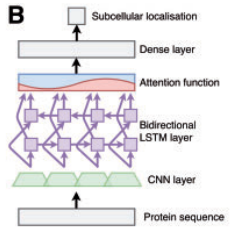
\includegraphics[width=0.4\linewidth]{subcellular}
\label{fig:subcellular}
\end{figure}

\subsection{Peptide MHCII}
"All neural networks were trained on the dataset used to develop NetMHCIIpan-3.0 (Karosiene et al., 2013). The dataset consists of 52,062 data points of peptide binding values measured as IC50/EC50 and covers 24 HLA-DR, 5 HLA-DP, 6 HLA-DQ and 2 mouse (H-2) molecules. Every MHCII molecule in the dataset is covered by at least 50 peptide binding measurements. The data were originally downloaded from the IEDB (Vita et al., 2015) and subsequently partitioned into five folds for the development of the NetMHCIIpan-3.0 method. The partitioned data are available for download at https://github.com/vanessajurtz/lasagne4bio. During partitioning care was taken to include all measurements of a single peptide against multiple MHC molecules in the same data partition.

The amino acids of the peptide sequence were encoded using a Blosum62 matrix. For the MHC molecules a pseudo sequence, consisting of amino acids that are in potential contact with a bound peptide, was derived as described by (Nielsen et al., 2008) and encoded using a Blosum62 matrix. The IC50/EC50 binding values were log transformed to fall in the 0-1 interval using the relation 1-log(IC50nM)/log(50,000).

The architecture of the convolutional neural networks is visualized in Figure 3B and Table S3. 1000, 1300, 1500 and 1700 convolutional filters of the size 9 amino acids were applied to the peptide sequence. Subsequently max pooling was performed to keep only the maximal activation of each filter over the complete peptide sequence and make the model invariant to peptide sequence length. The max pooling results were combined with the MHC pseudo sequence and fed into a dense (or fully connected) layer containing 60 hidden neurons. This layer feeds into the output layer. Rectifier nonlinearities (Maas et al., 2013) were applied to all hidden neurons and the sigmoid activation function to the output. All weights were initialized with glorot weights sampled from the uniform distribution (gain=0.05). To train the network, the squared error was calculated and the weights were updated using Adam updates (Kingma and Ba, 2014) with a learning rate of 0.0001 (β1 = 0.1, β2 = 0.001, epsilon= 10e-8). Batch normalization was applied to the input to all dense layers (Ioffe and Szegedy, 2015). All networks were trained for a total of 15 epochs using a mini-batch size of 20 examples.

To facilitate the distinction of peptide and MHC pseudo sequence, we encoded them in different input neurons. This means each amino acid was encoded in a vector with enough space for encoding 2 amino acids. If the amino acid was part of the peptide, it was encoded in the first part of the vector and the rest was set to zero, amino acids of the MHC pseudo sequence were encoded in the second part of the vector while the first part was set to zero. The input is fed into the LSTM layer (of either 100 or 120 LSTM units, depending on the architecture). The LSTM layer is connected to a dense layer containing 60 hidden neurons and the dense layer feeds into the output layer. The activation function of the LSTM layer was the hyperbolic tangent, rectify nonlinearities (Maas et al., 2013) were applied to the neurons of the dense layer and the sigmoid nonlinearity was applied to the output. All weights were initialized with glorot weights sampled from the uniform distribution (gain=0.05). To train the network the squared error was calculated and the weights were updated using Adam updates (Kingma and Ba, 2014) with a learning rate of 0.0001 (β1 = 0.1, β2 = 0.001, epsilon= 10e-8). Batch normalization was applied to the input to all dense layers (Ioffe and Szegedy, 2015). All networks were trained for a total of 150 epochs using a mini-batch size of 20 examples.

For each training partition, an ensemble containing 10 LSTMs with 100 LSTM units (trained on 10 different seeds), 10 LSTMs with 120 LSTM units, 5 CNNs with 1000 filters, 5 CNNs with 1300 filter, 5 CNNs with 1500 filters and 5 CNNs with 1700 filters. Trained using five fold cross validation, this amounts to a total of 200 networks (5*40), the same amount of networks as the NetMHCIIpan-3.0 ensemble. All trained CNN and LSTM neural networks were combined to an ensemble by calculating their average prediction. For the consensus method half the neural networks in the NetMHCIIpan ensemble (seeds 1-5) were combined with 10 LSTMs with 100 LSTM units, 5 CNNs with 1300 filters and 5 CNNs with 1500 filters.

CNN/LSTM:
Input layer (peptide/MHCII + peptide),
Conv: [9x21] 1000, 1300, 1500 or 1700 + Input layer (MHCII)/LSTM (100 or 120),
Batch normalization,
Dense (60),
Batch normalization,
Binding affinity
" \cite{Jurtz2017}
\begin{figure}[h]
	\centering
	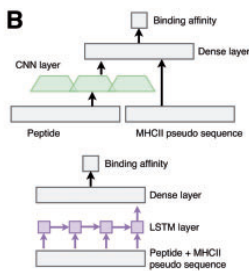
\includegraphics[width=0.4\linewidth]{mhcii}
\end{figure}

\subsection{Structural alphabet}
DeepCNF \cite{Wang2016}

\subsection{Backbone angles}
"There is a natural upper-bound on the maximum possible Q3 accuracy from inconsistencies in secondary structure assignment likely due to the coarseness and inherent arbitrariness of three-class labels (Kihara, 2005). This is likely also the case for the eight-class instantiation of the problem. A better approach might be to predict the sequence of back-bone angles for the amino acids, since these are experimentally observed values." \cite{Busia2017}

"Protein backbone structure can be described continuously by tor-
sion angles / and w. A number of methods have been developed to predict / and w as both discrete (Kuang et al.,2004; Kang et al., 1993) and continuous (Wood and Hirst, 2005; Dor and Zhou, 2007; Xue et al.,2008; Lyons et al.,2014) labels. More recently, a method (Lyons et al.,2014) was developed for predicting Ca atom-based h and s that describes the structure of four neighbouring residues, complement to the single residue structure described by / and w." \cite{Heffernan2017}

"a reduction of 5\%, 10\%, 5\% and 10\% in the mean absolute error for backbone /, w, h and s angles, respectively, [...] More significantly, 27\% of 182724 40-residue models directly constructed from predicted Ca atom-based h and s have similar structures to their corresponding native structures (6A˚ RMSD or less), which is 3\% better than models built by / and w angles." \cite{Heffernan2017}

"The ASA, /, w, h, s, HSE and CN prediction network uses square loss which is well suited to regres- sion problems (LeCun et al., 2006)." \cite{Heffernan2017}

"eight nodes for sin(/), cos(/), sin(w), cos(w), sin(h), cos(h), sin(s)and cos(s), respectively[...]. Utilizing the sine and cosine functions for angles is to remove the effect of the angle’s periodicity (Lyons et al.,2014). The sine and cosine predictions are converted back to angles by the equation a¼tan?1[sin(a)/ cos(a)]." \cite{Heffernan2017}

"The accuracy of /, w, h and s angles are measured as the Mean Absolute Error (MAE) between true and predicted angles. To compensate for the periodicity in angles, the error in the prediction of residue i is defined as the smaller of di and 360 ? di, where di is jApred i ?Atruej. Because both / and w have two peaks in their distributions, they can be split into two classes, where each class is defined as being closer to one of the two peaks. To evaluate large-angle errors the / angles are split into one state from [08 to 1508] and a second state made up of angles from [(1508 to 1808) and (?1808 to 08)]. The w angles are split into [?1008 to 608] for one state, and [(?1808 to ?1008) and (608 to 1808)] for the second." \cite{Heffernan2017}

\bibliography{bib}{}
\bibliographystyle{apalike}

\end{document}
